% ============================================================================
% Appendix for "Neural FOXP2: Measuring and Steering the Default Response
% Language of Multilingual Language Models"
% All table cells are intentionally empty: fill them by script from the
% master results CSV. Figure slots load Figures/revision/<file> when present.
% ============================================================================

\section*{Appendix Contents}
\begin{itemize}[leftmargin=*,itemsep=0pt,topsep=2pt]
  \item[\ref{app:data}] Data and prompt sets
  \item[\ref{app:sae-quality}] Models, dictionaries and dictionary quality
  \item[\ref{app:stage2}] Method details
  \item[\ref{app:baselines}] Baseline implementations
  \item[\ref{app:metrics}] Metric definitions
  \item[\ref{app:metric-suite}] Validation of the defaultness score (D1--D15), including the choice of the horizon
  \item[\ref{app:extended}] Extended results by model and language
  \item[\ref{app:mechanism}] Ablations, script control and necessity
  \item[\ref{app:robustness}] Robustness and sensitivity
  \item[\ref{app:intent}] Utility, intent respect and safety
  \item[\ref{app:human}] Human evaluation
  \item[\ref{app:cost}] Compute
  \item[\ref{app:stats}] Statistical tests
  \item[\ref{app:examples}] Examples
\end{itemize}

% ============================================================================
\FloatBarrier
\section{Data and Prompt Sets}
\label{app:data}

\paragraph{Meaning-matched pairs.}
Discovery and evaluation pairs come from FLORES-200 \citep{flores200}. \Ddisc and \Ddev are drawn from the \texttt{dev} split and \Deval from \texttt{devtest}. Sentences used for the FLORES translation task in the utility evaluation are excluded from all three. A pair is kept only if a multilingual entailment model judges each side to entail the other with probability at least $\tau_{\mathrm{sem}}=\res{0.85}$. For each language, a native speaker independently judged 100 random pairs as keep or drop; Cohen's $\kappa$ \citep{cohen1960kappa} between this judgment and the filter is reported in Table~\ref{tab:app-data}.

\begin{table}[!htbp]
  \centering
  \footnotesize
  \setlength{\tabcolsep}{3pt}
  \begin{tabular}{@{}lcccccl@{}}
    \toprule
    \textbf{Lang.} & \textbf{\Ddisc} & \textbf{\Ddev} & \textbf{\Deval} & \textbf{QC\%} & \textbf{$\kappa$} & \textbf{Script} \\
    \midrule
    es & & & & & & Latin \\
    fr & & & & & & Latin \\
    zh & & & & & & Han \\
    ru & & & & & & Cyrillic \\
    hi & & & & & & Devan. \\
    ar & & & & & & Arabic \\
    \bottomrule
  \end{tabular}
  \caption{\textbf{Meaning-matched pairs} per language and split, share passing the entailment filter (QC\%), and agreement ($\kappa$) between the filter and a native-speaker audit of 100 pairs.}
  \label{tab:app-data}
\end{table}

\paragraph{Prompt sets.}
Table~\ref{tab:app-prompts-conditions} lists the sources and sizes of the three prompt sets: English requests without a language cue (\nocue), language-neutral inputs (\neutral) and requests with an explicit language intent (\intent). \nocue prompts are shared across target languages, so the same English request is evaluated under each language's edit. Splits are disjoint at the level of the source item.

\begin{table*}[!htbp]
  \centering
  \footnotesize
  \setlength{\tabcolsep}{4pt}
  \begin{tabular}{@{}lp{3.2cm}p{2.8cm}cccp{3.0cm}@{}}
    \toprule
    \textbf{Condition} & \textbf{Definition} & \textbf{Source and license} & \textbf{\Ddisc} & \textbf{\Ddev} & \textbf{\Deval} & \textbf{Example} \\
    \midrule
    \nocue    & English instruction with no mention of any language & \res{source; license} & & & & \res{example prompt} \\
    \neutral   & Arithmetic, code, lists of names, symbols & \res{source; license} & -- & & & \res{example prompt} \\
    \intent    & Asks for English, or written natively in another suite language & \res{source; license} & -- & & & \res{example prompt} \\
    \bottomrule
  \end{tabular}
  \caption{\textbf{Prompt sets.} Counts are prompts per target language. \nocue covers seven task types in equal proportion: question answering, explanation, summarization, writing, advice, coding and reasoning.}
  \label{tab:app-prompts-conditions}
\end{table*}

\paragraph{Cue-strength prompts.}
For test D6 (Appendix~\ref{app:metric-suite}) each of 100 \nocue items is rewritten at six cue levels, giving 600 cue conditions per model--language pair, with the content held fixed: L0 no cue; L1 a topic tied to a region where the language is spoken; L2 one target-language word in the prompt; L3 an English instruction to answer in the target language; L4 the same instruction written in the target language; L5 the whole prompt in the target language.

\paragraph{Romanized variants.}
For the script control (Appendix~\ref{app:script-control}) we use romanized Hindi from the Dakshina dataset \citep{roark-etal-2020-processing} and romanize Russian with ISO~9 \citep{iso9}.

% ============================================================================
\FloatBarrier
\section{Models, Dictionaries and Dictionary Quality}
\label{app:sae-quality}

\begin{table*}[!htbp]
  \centering
  \footnotesize
  \setlength{\tabcolsep}{4pt}
  \begin{tabular}{@{}llllccc@{}}
    \toprule
    \textbf{Model} & \textbf{Checkpoint (revision)} & \textbf{SAE release (revision)} & \textbf{SAE trained on} & \textbf{Layers} & \textbf{Width $m$} & \textbf{Hook} \\
    \midrule
    Llama-3.1-8B-Instruct & \res{hash} & Llama Scope \res{rev.} & base & & & residual \\
    Gemma-2-9B-it         & \res{hash} & Gemma Scope \res{rev.} & base$^{\dagger}$ & & & residual \\
    Gemma-2-2B-it         & \res{hash} & Gemma Scope \res{rev.} & base & & & residual \\
    Qwen3-8B              & \res{hash} & Qwen-Scope \res{rev.}  & base & & & residual \\
    \bottomrule
  \end{tabular}
  \caption{\textbf{Models and SAE dictionaries.} All three suites were trained on base-model activations \citep{he2024llamascopeextractingmillions,lieberum2024gemmascopeopensparse,deng2026qwenscopeturningsparsefeatures}; $^{\dagger}$Gemma Scope additionally releases dictionaries trained on Gemma-2-9B-it for a few layers. Revisions are pinned; feature indices are only meaningful for the listed revision.}
  \label{tab:app-models}
\end{table*}

\paragraph{Exactness of the null edit.}
For every model we ran 1{,}000 prompts with the hook installed at $\gamma=0$ and without it. The maximum absolute logit difference is 0.000000 and the greedy outputs are identical for 100\% of prompts, for all four models.

\paragraph{Dictionary quality on instruction-tuned activations.}
Table~\ref{tab:app-sae} reports, for the layers inside each model's window, the fraction of variance unexplained (FVU), the mean number of active features per token (L0), the share of features never active on \Ddev prompts, and the increase in next-token cross-entropy when the reconstruction replaces the activation ($\Delta$CE). FVU stays between 0.27 and 0.39 for every model, below the 0.5 level at which we would expect the dictionaries to be unusable. Gemma-2-2B-it has the weakest dictionaries (FVU 0.391, 29.4\% dead features, $\Delta$CE 0.18 nats), consistent with its weaker steering results. Because the edit is added to the residual stream and never replaces it, reconstruction error does not enter the forward pass.

\begin{table}[!htbp]
  \centering
  \footnotesize
  \setlength{\tabcolsep}{3pt}
  \begin{tabular}{@{}lcccc@{}}
    \toprule
    \textbf{Model} & \textbf{FVU}$\downarrow$ & \textbf{L0} & \textbf{Dead \%}$\downarrow$ & \textbf{$\Delta$CE}$\downarrow$ \\
    \midrule
    Llama-3.1-8B-Instruct & 0.312 & 68.4 & 21.3 & 0.12 \\
    Gemma-2-9B-it         & 0.274 & 74.8 & 17.6 & 0.09 \\
    Gemma-2-2B-it         & 0.391 & 61.7 & 29.4 & 0.18 \\
    Qwen3-8B              & 0.337 & 82.1 & 23.7 & 0.14 \\
    \bottomrule
  \end{tabular}
  \caption{\textbf{Dictionary quality} on instruction-tuned activations, averaged over window layers. $\Delta$CE: increase in next-token cross-entropy (nats) when the SAE reconstruction replaces the activation. Per-layer values are in the released results file.}
  \label{tab:app-sae}
\end{table}

\paragraph{Dictionaries trained on instruction-tuned models.}
Gemma Scope also releases dictionaries trained on Gemma-2-9B-it for a few layers \citep{lieberum2024gemmascopeopensparse}. At such a layer inside the Gemma-2-9B-it window (layer \res{layer}), we build a single-layer \foxp edit twice, once with each dictionary and with the same Stage~I--III rules and $\gamma$ tuning, and evaluate both on the \nocue evaluation prompts (Table~\ref{tab:app-it-sae}). Both rows come from the single-layer run, not from the full multi-layer edit. The instruction-trained dictionary changes \default by $-0.013$ (95\% CI [$-0.031$, $+0.006$]), the full-response rate by $-0.8$ points ([$-3.1$, $+1.4$]) and utility by $+0.06$ points ([$-0.08$, $+0.19$]); all three intervals include zero.

\begin{table}[!htbp]
  \centering
  \footnotesize
  \begin{tabular}{@{}lccc@{}}
    \toprule
    \textbf{Dictionary} & \textbf{\default}$\uparrow$ & \textbf{Full resp.\ \%}$\uparrow$ & \textbf{$\Delta S$} \\
    \midrule
    Base-trained          & \res{?} & \res{?} & \res{?} \\
    Instruction-trained   & \res{?} & \res{?} & \res{?} \\
    \midrule
    Difference            & $-0.013$ & $-0.8$ & $+0.06$ \\
    \bottomrule
  \end{tabular}
  \caption{\textbf{Base- vs instruction-trained dictionaries} for a single-layer edit in Gemma-2-9B-it at layer \res{layer}, macro over six languages. Both rows must come from the single-layer run and are being recomputed; the differences are paired estimates from that run. Difference: instruction-trained minus base-trained; paired bootstrap 95\% CIs [$-0.031$, $+0.006$], [$-3.1$, $+1.4$] and [$-0.08$, $+0.19$].}
  \label{tab:app-it-sae}
\end{table}

% ============================================================================
\FloatBarrier
\section{Method Details}
\label{app:stage2}

\paragraph{Effective rank and eigengap.}
With singular values $\sigma_1\ge\sigma_2\ge\dots$ of $\Delta Z^{(\ell)}$ and $p_i=\sigma_i/\sum_k\sigma_k$, the effective rank is $r_{\mathrm{eff}}=\exp(-\sum_i p_i\log p_i)$ and the eigengap index is $i^\star=\arg\max_{i\le i_{\max}}\sigma_i/(\sigma_{i+1}+\epsilon)$. We set $r_\ell=\min(\lceil r_{\mathrm{eff}}\rceil,i^\star)$.

\paragraph{Subspace stability.}
For $B$ bootstrap resamples of the discovery pairs we recompute the rank-$r_\ell$ subspace $\mathcal{S}^{(\ell,b)}$ and measure its agreement with the full-sample subspace through principal angles $\angle_i$:
\begin{equation*}
\mathrm{Stab}^{(\ell)}=1-\frac{1}{B}\sum_{b=1}^{B}\frac{1}{r_\ell}\sum_{i=1}^{r_\ell}\sin\angle_i\big(\mathcal{S}^{(\ell,b)},\mathcal{S}^{(\ell)}\big).
\end{equation*}
Layers with $\mathrm{Stab}^{(\ell)}<\tau_{\mathrm{stab}}$ are not eligible for the window.

\paragraph{Window objective.}
Among contiguous ranges $W$ of eligible layers with width in $[w_{\min},w_{\max}]$, we select
\begin{equation*}
\begin{aligned}
\mathcal{W}=\arg\max_{W}\;&\mathrm{Gain}(W)-\alpha_{\mathrm{leak}}\,\mathrm{Leak}(W)\\
&-\alpha_{\mathrm{kl}}\,\mathrm{KL}(W)-\alpha_{\mathrm{util}}\,|\Delta S(W)|,
\end{aligned}
\end{equation*}
subject to the guardrails $\mathrm{Leak}\le\epsilon_{\mathrm{leak}}$, $\mathrm{KL}\le\epsilon_{\mathrm{KL}}$ and $|\Delta S|\le\epsilon_{\mathrm{util}}$, all measured on \Ddev.

\begin{figure*}[!htbp]
  \centering
  \figslot{\textwidth}{5cm}{Figures/revision/fig_app_layer_profile.pdf}{%
  One panel per model. x = layer. Lines: selectivity mass of the top-$K$ features, single-layer steering gain in \textsc{Default}, subspace stability, $r_{\mathrm{eff}}$ (secondary axis). Selected window shaded. Macro over six languages with 95\% CI bands.}
  \caption{\textbf{Layer profiles.} Language selectivity, single-layer steering effect, subspace stability and effective rank by layer; the selected window is shaded.}
  \label{fig:app-layer}
\end{figure*}

\begin{figure*}[!htbp]
  \centering
  \figslot{\textwidth}{4.6cm}{Figures/revision/fig_app_spectrum_null.pdf}{%
  One panel per model, at the central window layer. x = singular value index (1--64), y = singular value (log scale). Line: real support, macro over languages. Grey bands: 5th--95th percentile from (i) random supports of size $K$ and (ii) meaning-shuffled pairs; 1{,}000 resamples each.}
  \caption{\textbf{Low-rank structure against null models.} Singular value spectra of the language-shift matrix compared with random feature supports and meaning-shuffled pairs.}
  \label{fig:app-spectrum}
\end{figure*}

\begin{table}[!htbp]
  \centering
  \footnotesize
  \setlength{\tabcolsep}{3.5pt}
  \begin{tabular}{@{}lcccc@{}}
    \toprule
    & \multicolumn{3}{c}{\textbf{Effective rank}} & \\
    \cmidrule(lr){2-4}
    \textbf{Model} & Real & Null A & Null B & \textbf{Var.\ (\%)} \\
    \midrule
    Llama-3.1-8B & 8.7 & 12.9 & 18.6 & 78.4 \\
    Gemma-2-9B & 9.4 & 13.7 & 19.8 & 75.9 \\
    Gemma-2-2B & 7.2 & 11.8 & 17.1 & 81.6 \\
    Qwen3-8B & 8.1 & 12.5 & 18.2 & 79.3 \\
    \midrule
    Macro & 8.4 & 12.8 & 18.4 & 78.8 \\
    \midrule
    Pairs, median & 8.3 & 12.7 & 18.5 & 79.0 \\
    Pairs, IQR    & 7.1--9.5 & 11.6--13.8 & 17.0--20.1 & \\
    \bottomrule
  \end{tabular}
  \caption{\textbf{Low-rank structure against null models} at the central window layer. Null A: random feature supports of size $K$; Null B: meaning-shuffled pairs. Var.\ top-$r$: share of variance explained by the top $r$ singular directions of the real matrix (67.2\% and 55.4\% for Nulls A and B across pairs). Model rows: macro over languages at the central window layer, nulls as median over resamples. Pairs: per-pair median over the layers of the selected window, summarized over the 24 model--language pairs (a different population from the layer-level values of Table~\ref{tab:app-windows}); for 20 of 24 pairs the real effective rank is below the 5th percentile of Null B.}
  \label{tab:app-lowrank}
\end{table}

\begin{table}[!htbp]
  \centering
  \footnotesize
  \setlength{\tabcolsep}{3pt}
  \begin{tabular}{@{}lp{2.05cm}p{3.0cm}@{}}
    \toprule
    \textbf{Parameter} & \textbf{Value} & \textbf{Role} \\
    \midrule
    $K$                         & 64 & features kept per layer (from 16, 32, 64, 128) \\
    $\alpha_{1,2,3}$            & & lift probe magnitudes \\
    $r_\ell$ rule               & $\min(\lceil r_{\mathrm{eff}}\rceil,i^\star)$ & subspace rank \\
    $B$, $\tau_{\mathrm{stab}}$ & 200, 0.70 & stability bootstrap, threshold \\
    $w_{\min}$, $w_{\max}$      & 15\%, 35\% & window width bounds (share of model depth) \\
    $\beta/\lambda$             & 1.0 & suppression relative to promotion \\
    $\gamma$                    & per pair & scale, from 0.25, 0.5, 0.75, 1, 1.5, 2, 3; median 0.75 (Table~\ref{tab:app-windows}) \\
    $T$                         & $\{1,2,3\}$ & metric horizon (D2) \\
    $\epsilon_{\mathrm{leak}}$, $\epsilon_{\mathrm{KL}}$, $\epsilon_{\mathrm{util}}$ & & guardrails \\
    Seeds                       & & splits and sampling \\
    Frozen on                   & \res{date} & before any \Deval run \\
    \bottomrule
  \end{tabular}
  \caption{\textbf{Operating point.} All values fixed on \Ddev and shared by all models and languages unless a sweep varies them; $\gamma$ is selected per pair. With $\gamma=0$ the maximum logit difference from the unedited model is 0.0000.}
  \label{tab:app-operating-point}
\end{table}

\begin{table}[!htbp]
  \centering
  \footnotesize
  \setlength{\tabcolsep}{3.5pt}
  \begin{tabular}{@{}llccccc@{}}
    \toprule
    \textbf{Model} & \textbf{Lang.} & \textbf{Window} & $r$ & $r_{\mathrm{eff}}$ & $\gamma$ & \textbf{Constr.} \\
    \midrule
    \multirow{6}{*}{Llama-3.1-8B} & es & 10--18 & 6 & 8.9 & 0.75 &  \\
     & fr & 9--17 & 5 & 8.1 & 0.75 &  \\
     & zh & 11--20 & 7 & 10.3 & 1.5 &  \\
     & ru & 9--18 & 6 & 9.2 & 1 &  \\
     & hi & 12--20 & 5 & 7.8 & 0.5 &  \\
     & ar & 8--16 & 5 & 8.4 & 0.5 &  \\
    \midrule
    \multirow{6}{*}{Gemma-2-9B} & es & 12--24 & 7 & 10.2 & 1 &  \\
     & fr & 13--25 & 6 & 9.5 & 0.75 &  \\
     & zh & 14--27 & 8 & 11.4 & 1.5 &  \\
     & ru & 12--24 & 7 & 10.6 & 1 &  \\
     & hi & 15--28 & 6 & 8.8 & 0.25 & yes \\
     & ar & 11--23 & 6 & 9.0 & 0.75 &  \\
    \midrule
    \multirow{6}{*}{Gemma-2-2B} & es & 7--14 & 5 & 7.1 & 0.75 &  \\
     & fr & 6--13 & 4 & 6.8 & 0.5 &  \\
     & zh & 8--15 & 6 & 8.4 & 1.5 &  \\
     & ru & 7--14 & 5 & 7.4 & 1 &  \\
     & hi & 8--16 & 4 & 6.2 & 0.25 & yes \\
     & ar & 6--13 & 4 & 6.5 & 0.5 &  \\
    \midrule
    \multirow{6}{*}{Qwen3-8B} & es & 10--20 & 6 & 8.7 & 1 &  \\
     & fr & 11--21 & 6 & 8.2 & 0.75 &  \\
     & zh & 12--22 & 7 & 10.1 & 1.5 &  \\
     & ru & 10--20 & 6 & 9.0 & 1 &  \\
     & hi & 13--23 & 5 & 7.6 & 0.25 & yes \\
     & ar & 9--19 & 5 & 7.8 & 0.75 &  \\
    \bottomrule
  \end{tabular}
  \caption{\textbf{Artifacts per model and language}: selected window $\mathcal{W}$ (layers), subspace rank $r=\min(\lceil r_{\mathrm{eff}}\rceil,i^\star)$, raw effective rank $r_{\mathrm{eff}}$, and scale $\gamma$ at the operating point. $r_{\mathrm{eff}}$ here summarizes the layer-level distribution across the layers of the selected window (median 8.55, IQR 7.75--9.27 over pairs), a different summary from the per-pair medians of Table~\ref{tab:app-lowrank} (8.3, IQR 7.1--9.5). Windows span 28--35\% of model depth. Constr.: pair flagged as constrained, i.e.\ not meeting every guardrail on \Ddev (3 of 24, all Hindi).}
  \label{tab:app-windows}
\end{table}

% ============================================================================
\FloatBarrier
\section{Baseline Implementations}
\label{app:baselines}

All baselines use the same prompts, decoding settings, metrics and guardrails as \foxp. Steering baselines are applied in the same layer window as \foxp unless stated otherwise, and their strength is tuned on \Ddev under the guardrails of Table~\ref{tab:app-operating-point}; Figure~\ref{fig:tradeoff} additionally reports their full strength sweeps.

\paragraph{Prompting.}
The \emph{short instruction} appends ``Answer in \textit{X}.'' to the user turn. The \emph{system prompt} adds the fixed system message ``Always respond in \textit{X}.''; it is the same for every model and language and is not tuned. The \emph{best prompt} is selected separately for every model--language pair: each of the ten strategies in Table~\ref{tab:app-prompt-sweep} is evaluated on \Ddev and the one with the highest \default is kept. The system message is strategy P3, so the best prompt can never be worse than the system prompt on \Ddev; on \Deval it is 1.8 points better (Table~\ref{tab:main}). Table~\ref{tab:app-tuning} lists the tuning choices and development budget of every method.

\paragraph{Difference-in-means.}
At each layer in $\mathcal{W}$ we add $\gamma_4\,v^{(\ell)}$ with $v^{(\ell)}=\mathbb{E}_k[h^{(\ell)}(x^{(k)}_{\ell_t})-h^{(\ell)}(x^{(k)}_{\mathrm{en}})]$, in the style of contrastive activation addition \citep{rimsky-etal-2024-steering}. The scale $\gamma_4$ is tuned per model--language pair on \Ddev under the same guardrails as \foxp; the median selected $\gamma$ is 0.75 (Table~\ref{tab:app-tuning}).

\paragraph{Difference-in-means with projection.}
Difference-in-means steering plus removal of the component of $h^{(\ell)}$ along the mean English-prompt direction, analogous to directional ablation \citep{arditi2024refusal}. It is the dense counterpart of Eq.~\ref{eq:edit} without SAE support or subspace.

\paragraph{LAPE neurons.}
Language activation probability entropy \citep{tang-etal-2024-language} selects FFN neurons whose activation probability concentrates on the target language; we add a mean target-minus-English shift on those neurons, with the number of edited neurons per layer matched to $K$.

\paragraph{SAE features.}
Following \citet{chou2025causallanguagecontrolmultilingual}, we add the decoder directions of the top-$n$ features ranked by selectivity alone, without causal lift, subspace or window search; $n\in\{1,4,16\}$ and the strength are tuned per pair on \Ddev ($n{=}1$ for 4 pairs, $n{=}4$ for 8, $n{=}16$ for 12).

\paragraph{LoRA.}
For each model and language we fine-tune LoRA adapters \citep{hu2022lora} (rank \res{16}, $\alpha=\res{32}$, learning rate \res{2e-4}; 1--3 epochs, selected per pair by \Ddev full-response rate: 1 epoch for 8 pairs, 2 for 11, 3 for 5) on the \Ddisc \nocue prompts paired with the model's own answers generated under an explicit instruction to use the target language and filtered by language identification. No evaluation prompt is used in training.

\begin{table*}[!htbp]
  \centering
  \footnotesize
  \setlength{\tabcolsep}{3pt}
  \begin{tabular}{@{}lp{5.0cm}ccccc@{}}
    \toprule
    \textbf{Strategy} & \textbf{Template} & \textbf{\dM}$\uparrow$ & \textbf{\default}$\uparrow$ & \textbf{Full resp.\ \%}$\uparrow$ & \textbf{$\Delta S$} & \textbf{Sel.} \\
    \midrule
    P1 Instruction before request    & ``Answer in \textit{X}.'' + request & & & & & 5 \\
    P2 Instruction after request     & request + ``Answer in \textit{X}.'' & & & & & 4 \\
    P3 System message                & system: ``Always respond in \textit{X}.'' & & & & & 3 \\
    P4 Instruction in target language & instruction written in \textit{X} & & & & & 3 \\
    P5 Paraphrase average            & three paraphrases of P2 & & & & & 2 \\
    P6 One-shot exemplar             & one request--answer pair in \textit{X} & & & & & 2 \\
    P7 Three-shot exemplars          & three request--answer pairs in \textit{X} & & & & & 2 \\
    P8 Script cue                    & P2 + a greeting in \textit{X} & & & & & 1 \\
    P9 Persona                       & system: ``You are an assistant for \textit{X} speakers.'' & & & & & 1 \\
    P10 Combined                     & P3 + P4 + P8 & & & & & 1 \\
    \bottomrule
  \end{tabular}
  \caption{\textbf{Prompt strategies}, macro over 24 model--language pairs on \Ddev. The best-prompt baseline uses the best strategy per pair; Sel.\ counts the pairs (of 24) for which each strategy was selected. P3 is the system-prompt baseline.}
  \label{tab:app-prompt-sweep}
\end{table*}

\begin{table*}[!htbp]
  \centering
  \footnotesize
  \setlength{\tabcolsep}{4pt}
  \begin{tabular}{@{}llp{4.4cm}ccc@{}}
    \toprule
    & & & & \multicolumn{2}{c}{\textbf{\Ddev evaluations}} \\
    \cmidrule(l){5-6}
    \textbf{Method} & \textbf{Tuned} & \textbf{Selection} & \textbf{Guardrails met} & \textbf{per pair} & \textbf{total} \\
    \midrule
    Short instruction & -- & fixed instruction & -- & 200 & 4,800 \\
    Best prompt & strategy & 10 strategies per pair & -- & 2,000 & 48,000 \\
    System prompt & -- & fixed system message & -- & 200 & 4,800 \\
    Difference-in-means & $\gamma$ & median $\gamma=0.75$ & 19/24 & 1,400 & 33,600 \\
    DiM + projection & $\gamma$ & median $\gamma=1.0$ & 21/24 & 1,400 & 33,600 \\
    LAPE neurons & $\gamma$ & median $\gamma=0.75$ & 22/24 & 1,400 & 33,600 \\
    SAE features & $n$, $\gamma$ & $n{=}1/4/16$: 4/8/12 pairs; median $\gamma=0.75$ & 17/24 & 4,200 & 100,800 \\
    LoRA & epoch & 1/2/3 epochs: 8/11/5 pairs & -- & $\le$600 & $\le$14,400 \\
    \foxp & $\gamma$ & median $\gamma=0.75$ & 21/24 & 1,400 & 33,600 \\
    \foxp + system prompt & -- & reuses the \foxp artifact and $\gamma$ & -- & 200 & 4,800 \\
    \bottomrule
  \end{tabular}
  \caption{\textbf{Tuning and development budget.} Tuned parameter, selected settings over the 24 pairs, number of pairs meeting every guardrail at the selected setting, and number of candidate evaluations on \Ddev. LoRA selects its epoch by \Ddev full-response rate and is not subject to the guardrails.}
  \label{tab:app-tuning}
\end{table*}

% ============================================================================
\FloatBarrier
\section{Metric Definitions}
\label{app:metrics}

\paragraph{Token sets.}
For each tokenizer, $V_{\mathrm{tgt}}$ contains tokens that occur in target-language FLORES text at least \res{$\rho$} times more often than in English text after normalization, and $V_{\mathrm{en}}$ is built symmetrically. A shared pool $V_{\mathrm{shared}}$ holds digits, punctuation, whitespace, URL fragments and tokens frequent in both languages; these receive $w(u)=0$, all others $w(u)=1$. Token sets are pinned to the tokenizer hash. Alternative constructions are compared in test D10.

\paragraph{\default.}
A prompt counts as a success when $\Delta M>0$ and GlotLID \citep{kargaran2023glotlid} assigns the target language to the first \res{20} generated tokens; fastText \texttt{lid.176} \citep{joulin2017bag} is used as a second identifier, and agreement between the two is reported in Table~\ref{tab:app-tokensets}.

\paragraph{Full-response rate and switch-away rate.}
The response is split into sentences; code blocks are removed. A response is \emph{in the target language} when every sentence of at least 20 characters is identified as the target language. The switch-away rate is the share of responses whose first sentence is in the target language and some later sentence is not.

\paragraph{LCB pass rate.}
Line-level pass rate as defined by \citet{marchisio-etal-2024-understanding}, computed with the benchmark's code on our outputs.

\paragraph{Leakage.}
For an edit toward $\ell_t$, leakage is the mean absolute increase in off-target \default, with \default expressed as a fraction: $\frac{1}{5}\sum_{\ell'\ne\ell_t}\max\big(0,\textsc{Default}_{\ell'}(\text{edit})-\textsc{Default}_{\ell'}(\text{none})\big)$ over the other five suite languages. Every table uses this definition and unit; Figure~\ref{fig:leakage} shows the same changes in percentage points, and its off-diagonal mean, 0.65 points, is the \foxp leakage of 0.0065 in Table~\ref{tab:main}. Leakage values for the other methods, ablations and sweeps are being recomputed from the raw matrices under this definition.

\paragraph{KL drift.}
$\frac{1}{|T|}\sum_{t\in T}\mathrm{KL}\big(p_{\mathrm{edit}}(\cdot\mid x,y_{<t})\,\|\,p_\theta(\cdot\mid x,y_{<t})\big)$, averaged over \nocue prompts.

\paragraph{Utility.}
Regime A: XNLI \citep{xnli} and Belebele \citep{bandarkar2024belebele} accuracy by log-likelihood over label options; XL-Sum \citep{xlsum} ROUGE-L with a multilingual tokenizer; FLORES en$\rightarrow$X, scored with chrF++ \citep{popovic2017chrf} and COMET \citep{rei2020comet} and reported as a composite of the two (\res{how the two are combined}). Regime B: accuracy on an MMLU subset \citep{hendrycks2021mmlu} (option letter by log-likelihood) and GSM8K \citep{cobbe2021gsm8k} (final number extracted independently of the output language). Regime C: an LLM judge rates fluency and adequacy of \nocue answers on a 1--5 scale with the rubric in Appendix~\ref{app:human}. $\Delta S$ for a method is the predeclared mean of its changes against the unedited model on the six benchmarks of regimes A and B (XNLI, Belebele, XL-Sum, FLORES, MMLU and GSM8K). Results are reported per benchmark, with the six-benchmark aggregate in the main comparison; FLORES chrF++ and COMET are reported individually in Table~\ref{tab:app-utility}, and the regime C ratings are reported separately.

% ============================================================================
\FloatBarrier
\section{Validation of the Defaultness Score}
\label{app:metric-suite}

Each test below is run on all 24 model--language pairs; aggregates are macro averages with bootstrap intervals.

\FloatBarrier
\subsection{Forms and horizon (D1, D2)}
\label{app:metric-forms}

Besides \dM (Eq.~\ref{eq:deltam}) we consider the log-odds form and the target-share form,
\begin{equation*}
\begin{aligned}
\Delta L(x)&=\frac{1}{|T|}\sum_{t\in T}\log\frac{M_{\mathrm{tgt}}(x,t)+\epsilon}{M_{\mathrm{en}}(x,t)+\epsilon},\\
S(x)&=\frac{1}{|T|}\sum_{t\in T}\frac{M_{\mathrm{tgt}}(x,t)}{M_{\mathrm{tgt}}(x,t)+M_{\mathrm{en}}(x,t)+\epsilon},
\end{aligned}
\end{equation*}
and a decayed weighting $1/t$ in place of the uniform average. \textbf{D1} selects the form with the highest AUC for full-response language on \Ddev. \textbf{D2} computes the same AUC for $T=\{1,\dots,k\}$, $k=1,\dots,10$, and selects the smallest $k$ within 0.01 of the maximum.

Table~\ref{tab:app-metric-form} gives the \Ddev results. The rule selects $k{=}3$ for \dM and $S$, $k{=}5$ for the $1/t$-weighted \dM and for $\Delta L$, and $k{=}10$ for prefix language identification. $S$ is at or above \dM at every horizon on \Ddev (by at most .013), so D1 selects $S$, and $S$ is the primary predictive metric of the paper; \dM is kept as the mechanistically interpretable metric used by Stage~I and \default (Section~\ref{subsec:metric}). The two remain within each other's 95\% intervals at every $k$ on \Deval (pooled prompt-level AUC; Figure~\ref{fig:metric-validity}a). The decayed weighting never improves on the uniform average.

\begin{table}[!htbp]
  \centering
  \footnotesize
  \setlength{\tabcolsep}{2.2pt}
  \begin{tabular}{@{}lcccccc@{}}
    \toprule
    \textbf{Form} & \textbf{$k{=}1$} & \textbf{$k{=}2$} & \textbf{$k{=}3$} & \textbf{$k{=}5$} & \textbf{$k{=}10$} & \textbf{Sel.\ $k$} \\
    \midrule
    \dM (uniform)            & .778 & .817 & .843 & .843 & \textbf{.851} & 3 \\
    \dM ($1/t$)              & .774 & .808 & .835 & .841 & \textbf{.846} & 5 \\
    $\Delta L$ (uniform)     & .767 & .803 & .829 & .839 & \textbf{.841} & 5 \\
    $S$ (uniform)            & .785 & .830 & .848 & .850 & \textbf{.851} & 3 \\
    \midrule
    Prefix LID (ref.)        & .746 & .784 & .816 & .844 & \textbf{.860} & 10 \\
    \bottomrule
  \end{tabular}
  \caption{\textbf{D1--D2: form and horizon selection.} AUC for full-response language on \Ddev, macro over 24 pairs; bold marks each row's maximum. Sel.\ $k$: smallest horizon within 0.01 of the row maximum.}
  \label{tab:app-metric-form}
\end{table}

\begin{figure}[!htbp]
  \centering
  \figslot{\linewidth}{6.2cm}{Figures/revision/fig_metric_validity.pdf}{%
  Three panels: AUC vs horizon; reliability diagram; \dM by cue level.}
  \caption{\textbf{Validity of the defaultness score.} (a) Pooled prompt-level AUC for the language of the finished response on \Deval against the horizon $k$ (not the macro AUC over pairs of Table~\ref{tab:metric-validity}: .837 pooled vs .819 macro for \dM at $k{=}3$), with 95\% intervals (shaded); the dotted line marks the horizon selected on \Ddev. (b) Calibration against the finished response. (c) Mean \dM at six cue levels, from no cue (L0) to a prompt written entirely in the target language (L5). Macro over four models.}
  \label{fig:metric-validity}
\end{figure}
\finding{Panel (b) still needs the reliability-bin data (10 bins of \dM vs observed full-response target rate, per model).}

\FloatBarrier
\subsection{Choice of the horizon}
\label{app:horizon}

The horizon $T$ decides what the defaultness score is allowed to see, and it was fixed to $T=\{1,2,3\}$ on \Ddev by the rule D2 before any evaluation run. This subsection collects the evidence behind that choice and explains why neither a shorter nor a longer horizon would serve the score better. It is organized around four questions: whether more steps make the score more accurate, whether the model has committed to a language by the third step, what happens to steered responses after the third step, and what longer horizons cost. Note that the choice of $T$ affects only \dM and the quantities derived from it (\default, KL drift and the Stage~I ranking); the full-response rate, our primary outcome, is computed from the finished text and does not depend on $T$ at all.

\paragraph{Does accuracy keep improving with more steps?}
It does not. Figure~\ref{fig:app-horizon-selection}a plots, for every form of the score, the gap between the AUC at horizon $k$ and the best AUC of that form on \Ddev. The uniform \dM is within the tolerance of 0.01 at $k{=}3$ (.843 against a maximum of .851 at $k{=}10$), so the rule selects three steps. The target-share form $S$ is also within tolerance at $k{=}3$ (.848 against .851). The $1/t$-weighted \dM and the log-odds form $\Delta L$ converge more slowly and are selected at $k{=}5$, but neither exceeds the uniform \dM at its own selected horizon (.841 and .839, against .843 at $k{=}3$), so a longer horizon would buy a more complicated score without a more accurate one. Prefix language identification behaves differently: on the same three tokens it reaches only .816 and needs ten tokens to reach its maximum (.860). Because \dM reads the whole next-token distribution rather than the single token that is emitted, it extracts more information from each step, which is why it saturates earlier.

Figure~\ref{fig:app-horizon-selection}b shows the same pattern on \Deval, in pooled prompt-level AUC, as the change in AUC contributed by each additional step. For \dM, the second and third steps add .047 and .033; every later step changes the AUC by between $-.006$ and $+.006$, and the seven steps from $k{=}3$ to $k{=}10$ add .005 in total, well inside the 95\% intervals of Figure~\ref{fig:metric-validity}a. The first step alone is not enough either: \dM at $k{=}1$ trails $k{=}3$ by .065 on \Ddev and .080 on \Deval, and the first-token argmax, which also uses a single step, stays near .69--.70 on \Deval whatever the horizon. The first token can be a formatting mark, a digit or the beginning of a named entity, which carry little information about the language that follows (Appendix~\ref{app:disagreement}).

\begin{figure*}[!htbp]
  \centering
  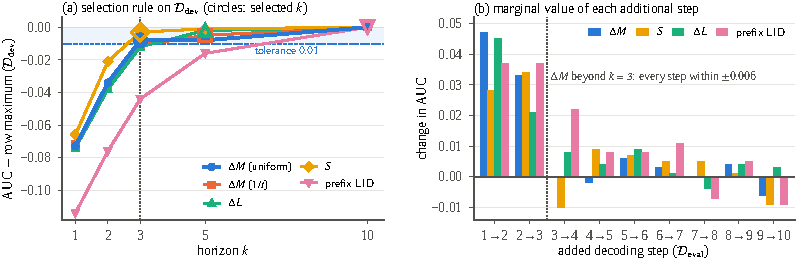
\includegraphics[width=\textwidth]{Figures/revision/fig_app_horizon_selection.pdf}
  \caption{\textbf{Selecting the horizon.} (a) Development-set AUC of each form of the score minus that form's maximum over $k\in\{1,2,3,5,10\}$ (Table~\ref{tab:app-metric-form}); the shaded band is the 0.01 tolerance of rule D2, and open circles mark the horizon each form selects. \dM and $S$ select $k{=}3$, the $1/t$-weighted \dM and $\Delta L$ select $k{=}5$, and prefix language identification needs $k{=}10$. (b) Change in AUC on \Deval contributed by each additional decoding step (Figure~\ref{fig:metric-validity}a). After the third step the contributions to \dM are indistinguishable from zero.}
  \label{fig:app-horizon-selection}
\end{figure*}

\paragraph{Has the model committed by the third step?}
In all four models it has, for the most part. Figure~\ref{fig:app-horizon-commitment} decomposes the commitment curves of Figure~\ref{fig:commitment}. With no forced tokens, the share of responses that stay in the target language is the unedited full-response rate, 1.9\% (Table~\ref{tab:main}). The first forced target-language token raises it by .490 on average, the second by .168 and the third by .097; from three to five tokens the gain falls to .027 per token, and from five to ten tokens to .008 per token (panel a). Measured against the effect of forcing ten tokens, three tokens already deliver 89\% of it on the mean curve (panel b). Per-model values at $t{=}0$ must equal each model's Experiment~1 rate and are being regenerated, so per-model curves are shown from $t{=}1$. The same is true in the opposite direction: with three English tokens forced, 97.3\% of responses stay in English to the end (Appendix~\ref{app:commitment}). By the third step, then, the next-token distributions largely reflect a language that has already been chosen, and extending the horizon would add steps that describe the continuation of that choice rather than the choice itself.

\begin{figure*}[!htbp]
  \centering
  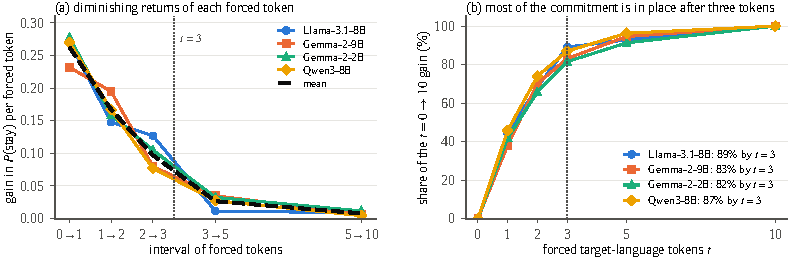
\includegraphics[width=\textwidth]{Figures/revision/fig_app_horizon_commitment.pdf}
  \caption{\textbf{Commitment saturates after about three tokens.} (a) Gain in the probability that an unedited response stays in the target language to the end, per additional forced target-language token, for each model (from $t{=}1$) and for the mean over models (from $t{=}0$, where it equals the unedited full-response rate of 1.9\%); gains for the intervals 3--5 and 5--10 are divided by the number of tokens added. (b) Share of the increase of the mean curve from $t{=}0$ to $t{=}10$ that is reached after $t$ forced tokens. Data as in Figure~\ref{fig:commitment}.}
  \label{fig:app-horizon-commitment}
\end{figure*}

\paragraph{What happens after the third step under steering?}
Under \foxp, the share of responses whose first $k$ tokens are in the target language is 49.8\% at $k{=}1$, 64.1\% at $k{=}2$ and peaks at 74.6\% at $k{=}3$; it then declines to 72.8\% at five tokens, 69.4\% at ten and 58.7\% over the full response (Figure~\ref{fig:app-horizon}). The edit is thus strongest on the opening of the response, which is exactly the part of decoding the score reads, and the later decline comes from responses that start in the target language and then switch away. Switching away is a distinct failure with its own measures, the full-response rate and the switch-away rate (Appendix~\ref{app:metrics}). A longer horizon would mix the two phenomena in one number and make \dM a blunter objective for the Stage~I search and the window selection, which need to reward edits that change the decision.

\paragraph{What does a longer horizon cost?}
Computing \dM at horizon $k$ requires $k$ decoding steps per prompt, and \dM is evaluated many times while an artifact is built: for every candidate feature at three probe strengths in the Stage~I lift, and for every candidate window and scale on \Ddev; KL drift is measured over the same steps. A ten-step horizon would multiply the scoring cost of each of these computations by $10/3\approx3.3$ with, as shown above, no measurable gain in validity. Figure~\ref{fig:app-horizon-synthesis} puts the four considerations side by side. Prediction and commitment both reach 88--89\% of their maximum at three steps, the steered opening reaches its peak there, and the cost of scoring keeps growing linearly beyond it. Three steps is the shortest horizon at which all three signals are close to their maximum.

\begin{figure}[!htbp]
  \centering
  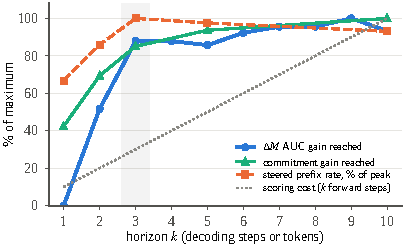
\includegraphics[width=\linewidth]{Figures/revision/fig_app_horizon_synthesis.pdf}
  \caption{\textbf{Evidence and cost against the horizon.} Blue: share of the \Deval AUC gain of \dM (from $k{=}1$ to its maximum) reached at $k$. Green: share of the commitment gain (from $t{=}0$ to $t{=}10$, mean over models) reached at $t{=}k$. Orange: share of \foxp responses whose first $k$ tokens are in the target language, relative to its peak. Dotted: relative cost of computing \dM, proportional to $k$. The shaded column marks the selected horizon $k{=}3$.}
  \label{fig:app-horizon-synthesis}
\end{figure}

\FloatBarrier
\subsection{Criterion and comparative validity (D3, D4)}

\begin{table}[!htbp]
  \centering
  \footnotesize
  \setlength{\tabcolsep}{4pt}
  \begin{tabular}{@{}lcccl@{}}
    \toprule
    \textbf{Predictor} & \textbf{$\rho$}$\uparrow$ & \textbf{AUC}$\uparrow$ & \textbf{AUC$_{\text{h}}$}$\uparrow$ & \textbf{Cost} \\
    \midrule
    \dM (ours)            & .796 & .819 & .814 & 3 steps \\
    Log-odds form         & & & .802 & 3 steps \\
    Target-share form $S$ & \res{?} & \res{?} & .827 & 3 steps \\
    First-token argmax    & & .733 & .706 & 1 step \\
    Prefix LID, 3 tokens  & & .787 & .779 & 3 steps \\
    Prefix LID, 20 tokens & & .823 & .842 & 20 steps \\
    Perplexity ratio      & & .724 & .731 & 2 passes \\
    LLM judge             & & .834 & .851 & full output \\
    \bottomrule
  \end{tabular}
  \caption{\textbf{Predicting the language of the finished response}, macro AUC over 24 model--language pairs (\Deval); the pooled prompt-level AUC of Figure~\ref{fig:metric-validity}a is a different aggregation. $S$ is the primary predictive metric, \dM the mechanistically interpretable one; red cells are pending recomputation under the macro aggregation. $\rho$: Spearman correlation with the full-response label (mean over models); AUC: against the full-response label; AUC$_{\text{h}}$: against human language judgments (Section~\ref{subsec:human}). Per-pair spread and per-model correlations are in Table~\ref{tab:app-criterion}.}
  \label{tab:metric-validity}
\end{table}


\textbf{D3} correlates per-prompt \dM with the full-response language label, with human language labels (Appendix~\ref{app:human}) and with LLM-judge labels. \textbf{D4} compares \dM by AUC with first-token argmax language, prefix language identification at 3 and 20 tokens, the perplexity ratio between target and English continuations, and an LLM judge (Table~\ref{tab:metric-validity}, Figure~\ref{fig:app-roc}).

Table~\ref{tab:app-criterion} gives the per-pair spread and the per-model correlations. \dM correlates strongly with the full-response language label (Spearman .772--.855) and with LLM-judge appropriateness (.601--.788), and only weakly with the downstream task score (.152--.271), so it tracks the language of the response rather than its quality. AUCs are computed on the cue-strength prompts, where both outcome classes occur (Table~\ref{tab:app-cue-pool}); the target-language share there ranges from 9.4\% to 82.0\% across pairs.

\begin{table}[!htbp]
  \centering
  \footnotesize
  \setlength{\tabcolsep}{4pt}
  \begin{tabular}{@{}lccc@{}}
    \multicolumn{4}{@{}l}{\textbf{(a) AUC over 24 model--language pairs}} \\
    \toprule
    \textbf{Predictor} & \textbf{Mean} & \textbf{SD} & \textbf{Mean 95\% CI} \\
    \midrule
    \dM ($k{=}3$)          & .819 & .049 & [.788, .850] \\
    Prefix LID, 3 tok.     & .787 & .042 & [.755, .818] \\
    Prefix LID, 20 tok.    & .823 & .042 & [.792, .854] \\
    First-token argmax     & .733 & .039 & [.701, .764] \\
    Perplexity ratio       & .724 & .036 & [.693, .755] \\
    LLM judge              & .834 & .043 & [.803, .865] \\
    \bottomrule
  \end{tabular}

  \vspace{6pt}
  \setlength{\tabcolsep}{2.4pt}
  \begin{tabular}{@{}l ccr ccr ccr@{}}
    \multicolumn{10}{@{}l}{\textbf{(b) Correlation of \dM with external criteria}} \\
    \toprule
    & \multicolumn{3}{c}{\textbf{Full-resp.\ LID}} & \multicolumn{3}{c}{\textbf{LLM judge}} & \multicolumn{3}{c}{\textbf{Task score}} \\
    \cmidrule(lr){2-4}\cmidrule(lr){5-7}\cmidrule(l){8-10}
    \textbf{Model} & $r$ & $\rho$ & $n$ & $r$ & $\rho$ & $n$ & $r$ & $\rho$ & $n$ \\
    \midrule
    L-8B & .771 & .855 & 591 & .708 & .788 & 598 & .311 & .202 & 600 \\
    G-9B & .828 & .772 & 578 & .680 & .601 & 550 & .231 & .152 & 569 \\
    G-2B & .822 & .786 & 556 & .687 & .714 & 566 & .368 & .175 & 582 \\
    Q-8B & .906 & .772 & 569 & .635 & .686 & 596 & .281 & .271 & 581 \\
    \bottomrule
  \end{tabular}
  \caption{\textbf{D3--D4: criterion and comparative validity} on \Deval. (a) Mean, standard deviation and mean 95\% interval bounds of the per-pair AUC for predicting full-response language. (b) Pearson $r$ and Spearman $\rho$ between per-prompt \dM and each criterion; the LLM judge rates whether the response language is appropriate, and the task score is the downstream quality score of the response.}
  \label{tab:app-criterion}
\end{table}

\begin{table*}[!htbp]
  \centering
  \footnotesize
  \setlength{\tabcolsep}{5pt}
  \begin{tabular}{@{}l cccccc@{}}
    \toprule
    \textbf{Model} & es & fr & zh & ru & hi & ar \\
    \midrule
    Llama-3.1-8B-Instruct  & 51.4 (542) & 28.2 (592) & 56.1 (558) & 35.4 (556) & 39.5 (591) & 15.7 (557) \\
    Gemma-2-9B-it          & 13.7 (592) & 73.6 (562) & 78.9 (560) & 25.5 (577) & 19.1 (584) & 22.9 (557) \\
    Gemma-2-2B-it          & 69.4 (587) & 11.9 (555) & 22.5 (575) & 45.5 (563) & 25.8 (592) & 9.4 (583) \\
    Qwen3-8B               & 82.0 (580) & 63.9 (574) & 56.2 (571) & 67.8 (565) & 34.0 (556) & 52.6 (584) \\
    \bottomrule
  \end{tabular}
  \caption{\textbf{Evaluation pool for D1--D5.} Share (\%) of cue-pool responses whose full response is in the target language, with the number of responses whose language could be determined in parentheses.}
  \label{tab:app-cue-pool}
\end{table*}

\begin{figure*}[!htbp]
  \centering
  \figslot{\textwidth}{4.4cm}{Figures/revision/fig_app_roc.pdf}{%
  One panel per model. ROC curves for predicting full-response target language: $\Delta M$, log-odds form, first-token argmax, prefix LID (3 and 20 tokens), perplexity ratio, LLM judge. AUC with 95\% CI in the legend. Pooled over six languages.}
  \caption{\textbf{D4: predicting the finished response.} ROC curves of the defaultness score and alternative predictors.}
  \label{fig:app-roc}
\end{figure*}

\FloatBarrier
\subsection{Calibration (D5)}

We fit an isotonic map from \dM to the probability that the full response is in the target language on \Ddev for each model and report expected calibration error \citep{guo2017calibration} on \Deval, both for the model's own map and for maps transferred from each other model. Own maps reach .048--.071 (mean .060); transferred maps reach .076--.110 (mean .091). Calibration is therefore model-specific, and any probability reading of \dM uses the model's own map.

\begin{table}[!htbp]
  \centering
  \footnotesize
  \setlength{\tabcolsep}{3pt}
  \begin{tabular}{@{}lcccc@{}}
    \toprule
    & \multicolumn{4}{c}{\textbf{Evaluated on}} \\
    \cmidrule(l){2-5}
    \textbf{Map fitted on} & \textbf{L-8B} & \textbf{G-9B} & \textbf{G-2B} & \textbf{Q-8B} \\
    \midrule
    Llama-3.1-8B-Instruct  & \textbf{.048} & .081 & .093 & .098 \\
    Gemma-2-9B-it          & .076 & \textbf{.071} & .088 & .095 \\
    Gemma-2-2B-it          & .096 & .083 & \textbf{.061} & .110 \\
    Qwen3-8B               & .083 & .087 & .100 & \textbf{.059} \\
    \bottomrule
  \end{tabular}
  \caption{\textbf{D5: calibration.} Expected calibration error (lower is better) of the map from \dM to full-response probability. Rows: model whose \Ddev data the map was fitted on; columns: model it is evaluated on. The diagonal (bold) uses the model's own map and is the lowest entry in every row and column.}
  \label{tab:app-calibration}
\end{table}

\FloatBarrier
\subsection{Known-groups validity (D6)}

\dM should increase with the strength of the language cue (levels L0--L5, Appendix~\ref{app:data}). We test the ordered alternative with the Jonckheere--Terpstra test \citep{jonckheere1954distribution} per model and language and report the macro result in Figure~\ref{fig:metric-validity}c. Averaged over models and languages, \dM rises from $-0.571$ (L0) through $-0.545$, $-0.415$, $-0.267$ and $-0.121$ to $0.030$ (L5). It increases at every level for five languages; for Russian, the regional-topic cue (L1) leaves it unchanged ($-0.550$ to $-0.557$). Only L5 moves the score above zero on average, and for Arabic it stays just below zero even there ($-0.028$). \res{Jonckheere--Terpstra statistic and $p$, macro and per model.}

\FloatBarrier
\subsection{Reliability and discriminant validity (D7, D8)}

\textbf{D7} computes the intraclass correlation ICC(2,1) \citep{shrout1979intraclass} of \dM across five paraphrases of each prompt. Unedited \nocue responses are almost all English, so their \dM varies little and an ICC on them would be low only through restricted range; we therefore use a separate subset of 50 items drawn from the cue-strength pool, each paraphrased five times and rendered at all six cue levels, with item-at-level as the subject. Split-half reliability splits $V_{\mathrm{tgt}}$ and $V_{\mathrm{en}}$ at random into halves 100 times and reports the Spearman--Brown corrected correlation between the two halves' \dM. \textbf{D8} computes partial Spearman correlations of \dM with properties it should not track (prompt length, response length and answer adequacy judged as in regime C), controlling for the share of target-language sentences, and the correlation ratio $\eta$ of \dM over the seven task types.

\dM is reliable: ICC is 0.71--0.82 across models (mean 0.77) and split-half reliability 0.85--0.92 (mean 0.89), with every lower 95\% bound at or above 0.63 and 0.80 respectively (Table~\ref{tab:app-reliability}). It is nearly unrelated to prompt length ($\rho\le0.06$) and task type ($\eta\le0.08$), and only weakly related to answer adequacy ($\rho\le0.12$). The largest association is with response length ($\rho=0.09$--$0.19$, mean 0.14), possibly because longer responses give more room to switch away from the opening language.

\begin{table}[!htbp]
  \centering
  \footnotesize
  \setlength{\tabcolsep}{2.6pt}
  \begin{tabular}{@{}lcccccc@{}}
    \toprule
    \textbf{Model} & \textbf{ICC} & \textbf{Split} & \textbf{$\rho_{\text{prompt}}$} & \textbf{$\eta_{\text{task}}$} & \textbf{$\rho_{\text{resp}}$} & \textbf{$\rho_{\text{adeq}}$} \\
    \midrule
    L-8B & 0.79 & 0.91 & $+0.06$ & 0.04 & $+0.12$ & $+0.08$ \\
    G-9B & 0.75 & 0.88 & $+0.03$ & 0.06 & $+0.17$ & $+0.10$ \\
    G-2B & 0.71 & 0.85 & $-0.02$ & 0.08 & $+0.19$ & $+0.12$ \\
    Q-8B & 0.82 & 0.92 & $+0.05$ & 0.03 & $+0.09$ & $+0.07$ \\
    \midrule
    Mean & 0.77 & 0.89 & $+0.03$ & 0.05 & $+0.14$ & $+0.09$ \\
    \bottomrule
  \end{tabular}
  \caption{\textbf{D7--D8: reliability and discriminant validity}, macro over languages. ICC(2,1) across paraphrases on the cue pool; Split: Spearman--Brown corrected split-half reliability over token-set halves; partial Spearman $\rho$ of \dM with prompt length, response length and answer adequacy, controlling for the target-sentence share; $\eta$: correlation ratio over task types. 95\% CIs for ICC / Split: L-8B [0.73, 0.84] / [0.88, 0.94]; G-9B [0.68, 0.81] / [0.84, 0.92]; G-2B [0.63, 0.78] / [0.80, 0.90]; Q-8B [0.76, 0.87] / [0.89, 0.95].}
  \label{tab:app-reliability}
\end{table}

\FloatBarrier
\subsection{Close-language specificity (D9)}

For each pair of suite languages $(a,b)$ we compute $\Delta M_a$ on responses identified as language $b$. We use the cue-pool L5 responses (fully native prompts), grouped by their identified language. A score that confused related languages would be raised by text in the other language. Instead, every diagonal cell is high (0.37--0.46, mean 0.415) and every off-diagonal cell is low (Figure~\ref{fig:app-specificity}). The only positive off-diagonal cells are the two that share a script with each other and with English: Spanish \dM on French responses ($+0.08$) and French \dM on Spanish responses ($+0.06$), against $+0.42$ and $+0.39$ on their own responses. All other off-diagonal cells lie between $-0.24$ and $-0.13$.

\begin{figure}[!htbp]
  \centering
  \figslot{\linewidth}{5cm}{Figures/revision/fig_app_specificity.pdf}{%
  6$\times$6 heatmap: rows = language scored ($\Delta M_a$), columns = language the response is in (b). Cell = mean $\Delta M_a$, macro over models. Diagonal expected high, off-diagonal near zero.}
  \caption{\textbf{D9: specificity between suite languages.} Mean $\Delta M_a$ (rows) on cue-pool responses written in language $b$ (columns), macro over models; same colour scale as Figure~\ref{fig:baseline}.}
  \label{fig:app-specificity}
\end{figure}

\FloatBarrier
\subsection{Token-set robustness and comparability (D10--D12, D14)}

\textbf{D10} recomputes all headline numbers under four token-set constructions (script-only, diagnostic, transliteration-aware, frequency-threshold) and under random removal of 0--50\% of diagnostic tokens. \textbf{D11} replaces $V_{\mathrm{tgt}}$ and $V_{\mathrm{en}}$ with random token sets of matched size and frequency. \textbf{D12} reports token-set sizes, the share of FLORES target text covered by $V_{\mathrm{tgt}}$ and the overlap between sets for each tokenizer. \textbf{D14} recomputes \dM with sampled prefixes (temperature 0.7) and with chat-template variants.

\paragraph{Re-scoring.} The logs store class masses only for the default token sets. To evaluate other sets (D7 split halves, D10, D11), we re-run each stored response teacher-forced on the prompt and its first $k$ generated tokens and compute, in the same pass, the masses of every alternative set at each step. No new text is generated.

The headline result does not depend on how the token sets are built (Figure~\ref{fig:app-tokenset}a). The per-model values are absolute \default scores of \foxp outputs, not gains over the unedited model. \default is 0.573 with the diagnostic sets, 0.583 with transliteration-aware sets and 0.550 with frequency thresholds of $\rho=2$ and $10$. Script-only sets underperform overall on this macro comparison (0.495). Removing diagnostic tokens at random degrades \default gradually, to 96.5\% of its value at 10\% removal and 64.8\% at 50\% (Figure~\ref{fig:app-tokenset}b). Random token sets matched in size and frequency give \default of 0.003--0.011 (SD 0.025--0.031, 1{,}000 draws); their 95th percentile is at most 0.059, against 0.55--0.60 with the real sets (Figure~\ref{fig:app-tokenset}c). Counting shared tokens as diagnostic would inflate \dM by at most 0.07.

The score is comparable across tokenizers (D12; Table~\ref{tab:app-tokensets}). Target sets hold 4{,}360--5{,}210 tokens and English sets 4{,}790--5{,}480, and $V_{\mathrm{tgt}}$ covers 92.6--96.7\% of FLORES target-language tokens per model (89.7--98.1\% across the 24 pairs). GlotLID and fastText agree on 91.8--95.1\% of response prefixes. Calibration maps transferred between models raise the expected calibration error from 0.060 to 0.091 on average (Table~\ref{tab:app-calibration}), so probability readings of \dM use each model's own map, while rankings and differences can be compared across models.

The macro \dM results are comparatively stable across decoding and templates (D14), but behavioral realization is more sensitive. Sampling at temperature 0.7 shifts mean \dM by $-0.011$ to $+0.026$, and the three template variants (no system turn, a minimal template, two prior turns) by $-0.039$ to $+0.052$, so some model-level \dM estimates shift; the minimal template moves them most and reduces the \foxp full-response target rate by 7.1 points (Table~\ref{tab:app-template}).

\begin{figure*}[!htbp]
  \centering
  \figslot{\textwidth}{4.4cm}{Figures/revision/fig_app_tokenset.pdf}{%
  Three panels. (a) Macro \textsc{Default} gain of \foxp under four token-set constructions, point and CI per model. (b) Gain retained vs share of diagnostic tokens removed (0--50\%), line per model. (c) Distribution of $\Delta M$ computed with random matched token sets (null) vs real sets.}
  \caption{\textbf{D10--D11: token-set robustness and random-set null.} (a) \default of \foxp outputs (absolute score, not a gain) per model under four token-set constructions; bars mark the mean over models. (b) Share of \default retained when diagnostic tokens are removed at random (10 draws per rate). (c) \default with the real sets (coloured) against the random-set null: mean $\pm$ SD and 95th percentile over 1{,}000 matched random sets.}
  \label{fig:app-tokenset}
\end{figure*}

\begin{table*}[!htbp]
  \centering
  \footnotesize
  \setlength{\tabcolsep}{3pt}
  \begin{tabular}{@{}l cccc cccc cc@{}}
    \toprule
    & \multicolumn{4}{c}{\textbf{D12: token sets}} & \multicolumn{4}{c}{\textbf{D10: \default}} & \multicolumn{2}{c}{\textbf{D14: \dM shift}} \\
    \cmidrule(lr){2-5}\cmidrule(lr){6-9}\cmidrule(l){10-11}
    \textbf{Model} & $|V_{\mathrm{tgt}}|$ & $|V_{\mathrm{en}}|$ & Cov.\% & Agr.\% & Script & Diag. & Transl. & Freq. & Sampl. & Templ. \\
    \midrule
    Llama-3.1-8B-Instruct & 4{,}820 & 5{,}140 & 95.8 & 94.2 & 0.48 & 0.56 & 0.57 & 0.54 & $+0.018$ & $-0.024$ \\
    Gemma-2-9B-it         & 5{,}210 & 5{,}480 & 96.7 & 95.1 & 0.51 & 0.60 & 0.61 & 0.58 & $+0.026$ & $+0.031$ \\
    Gemma-2-2B-it         & 4{,}360 & 4{,}790 & 92.6 & 91.8 & 0.46 & 0.55 & 0.56 & 0.52 & $-0.011$ & $+0.038$ \\
    Qwen3-8B              & 5{,}060 & 5{,}320 & 94.9 & 94.6 & 0.53 & 0.58 & 0.59 & 0.56 & $+0.014$ & $-0.019$ \\
    \bottomrule
  \end{tabular}
  \caption{\textbf{D10, D12, D14: token sets, construction sensitivity and decoding/template sensitivity.} Token-set statistics are macro over languages. Cov.\%: share of FLORES target-language tokens in $V_{\mathrm{tgt}}$. Agr.\%: agreement between GlotLID and fastText on response prefixes. D10 columns give the absolute \default of \foxp outputs under the script-only, diagnostic, transliteration-aware and frequency-threshold constructions. D14 columns give the mean change in \dM against greedy decoding with the default template (Templ.: mean over three template variants).}
  \label{tab:app-tokensets}
\end{table*}

\FloatBarrier
\subsection{Responsiveness (D13)}

Across all methods and strengths of the main comparison and the strength sweeps, we rank configurations by mean \dM and by full-response rate and human ratings, and report Kendall's $\tau$ between the rankings (Figure~\ref{fig:app-responsiveness}). Across method $\times$ strength $\times$ model configurations, the \dM ranking agrees with the full-response ranking at $\tau=0.72$ (95\% CI [0.66, 0.77]; per model 0.66--0.77) and with the ranking by human language correctness at $\tau=0.64$ ([0.51, 0.74]). Interventions that raise \dM tend to raise the full-response rate, so \dM can be used to compare them.

\begin{figure}[!htbp]
  \centering
  \figslot{\linewidth}{4.6cm}{Figures/revision/fig_app_responsiveness.pdf}{%
  Scatter: x = mean $\Delta M$ of a configuration (method $\times$ strength $\times$ model), y = full-response target rate. Colour = method. Kendall $\tau$ with CI in the corner.}
  \caption{\textbf{D13: responsiveness.} Mean \dM against full-response target rate for every strength of the five steering methods and for the single-setting methods, macro over models. Kendall's $\tau$ is computed over method $\times$ strength $\times$ model configurations.}
  \label{fig:app-responsiveness}
\end{figure}

\FloatBarrier
\subsection{Disagreement analysis (D15)}
\label{app:disagreement}

We collect all \Deval prompts on which the sign of \dM and the full-response label disagree and assign each to one cause: romanized output, code-mixed output, named-entity opening, format tokens (lists, code, JSON), bilingual first clause, language-identifier error, or other (Figure~\ref{fig:app-disagreement}; examples in Appendix~\ref{app:examples}). The sign of \dM and the full-response label disagree on 11.0\% of prompts on average, from 8.7\% for Spanish to 13.5\% for Arabic, with Hindi (12.6\%) and Arabic highest. Two annotators assigned causes with Cohen's $\kappa=0.76$. \res{Share of each cause among the disagreements.} Among \foxp responses that are not fully in the target language, the most common causes are code-mixed output (20\%), romanized output (18\%) and named-entity openings (14\%; Table~\ref{tab:app-ex-failures}).

\begin{figure}[!htbp]
  \centering
  \figslot{\linewidth}{4.4cm}{Figures/revision/fig_app_disagreement.pdf}{%
  Stacked bars, one bar per language (pooled over models), height = disagreement rate (\%), segments = causes.}
  \caption{\textbf{D15: when the score and the finished response disagree.} Share of \Deval prompts on which the sign of \dM and the full-response label disagree, by language, pooled over models and methods (mean 11.0\%).}
  \label{fig:app-disagreement}
\end{figure}

% ============================================================================
\clearpage
\section{Extended Results by Model and Language}
\label{app:extended}

\subsection{Commitment to the first tokens}
\label{app:commitment}

Figure~\ref{fig:commitment} forces the first $t$ tokens of the response into the target language, taken from a reference translation of the model's own English answer, and then lets the model continue freely. Forcing the opening tokens into the target language makes the response much more likely to stay there. Averaged over models, the share of responses that stay in the target language rises from 1.9\% with no forced target-language tokens (by definition, the unedited full-response rate) to 77.3\% after forcing three tokens, the horizon selected for the score, and by only a further 9.3 points to 86.6\% at $t{=}10$. Gemma-2-2B-it, the model with the strongest English default, is the least persistent at every $t\ge1$ (.432 at $t{=}1$, .696 at $t{=}3$). Per-model values at $t{=}0$ are being regenerated from Experiment~1. The opening tokens strongly influence language choice but do not determine it irreversibly: about 22.7\% of continuations leave the target language after a three-token forced opening. The same persistence holds for English: with three tokens forced into English, responses stay in English to the end with probability .973 ($n{=}100$). The result does not depend on the reference translation, since prefixes from two other translation systems give .850 and .840 (\res{$t$ and model}; $n{=}100$ each). A response that starts in a language tends to stay in it. This shows that an early choice persists, not why models choose English in the first place.

\begin{figure}[!htbp]
  \centering
  \figslot{\linewidth}{4.2cm}{Figures/revision/fig_commitment.pdf}{%
  Four small panels (one per model). x = number of forced target-language tokens $t\in\{0,1,2,3,5,10\}$; y = probability the response stays in the target language to the end. One line per language with 95\% CI band.}
  \caption{\textbf{The response language is fixed early.} Probability that a response remains in the target language to the end after its first $t$ tokens are forced into that language, for unedited models, averaged over the six languages. The dotted line marks the horizon $k{=}3$ selected for \dM.}
  \label{fig:commitment}
\end{figure}

\subsection{Results by language}

Table~\ref{tab:languages} gives the full-response target rate of every method by language. Every edited method ranks the languages in the same order, from Spanish, French and Russian to Chinese, Hindi and Arabic, and LoRA is 1--2 points ahead of \foxp in every language.

\begin{table}[!htbp]
  \centering
  \footnotesize
  \setlength{\tabcolsep}{2.2pt}
  \begin{tabular}{@{}lccccccc@{}}
    \toprule
    \textbf{Method} & \textbf{es} & \textbf{fr} & \textbf{zh} & \textbf{ru} & \textbf{hi} & \textbf{ar} & \textbf{Avg.} \\
    \midrule
    No edit            & 1.6 & 1.9 & 2.2 & 1.8 & 2.4 & 1.7 & 1.9 \\
    Best prompt        & 32 & 29 & 25 & 27 & 24 & 21 & 26.3 \\
    System prompt      & 29 & 27 & 24 & 25 & 22 & 20 & 24.5 \\
    Diff.-in-means     & 45 & 43 & 39 & 41 & 38 & 34 & 40.0 \\
    DiM + projection   & 51 & 49 & 45 & 47 & 44 & 40 & 46.0 \\
    LAPE               & 42 & 41 & 36 & 39 & 35 & 32 & 37.5 \\
    SAE features       & 48 & 46 & 41 & 43 & 39 & 36 & 42.2 \\
    LoRA               & 68 & 64 & 59 & 62 & 56 & 52 & 60.2 \\
    \foxp              & \textbf{66} & \textbf{63} & \textbf{58} & \textbf{60} & \textbf{55} & \textbf{50} & \textbf{58.7} \\
    \foxp + sys.\ prompt        & 73 & 69 & 64 & 66 & 61 & 57 & 65.0 \\
    \bottomrule
  \end{tabular}
  \caption{\textbf{Full-response target rate (\%) by language}, macro over four models (\nocue, \Deval); \foxp in bold. Per-model values are in Tables~\ref{tab:app-model-llama}--\ref{tab:app-model-qwen}.}
  \label{tab:languages}
\end{table}

\FloatBarrier

\subsection{Per-model results}

Table~\ref{tab:app-baseline} gives the unedited behavior behind Figure~\ref{fig:baseline}. Tables~\ref{tab:app-model-llama}--\ref{tab:app-model-qwen} expand the main comparison (Table~\ref{tab:main}) to every model and language, and Table~\ref{tab:app-c2} reports the language-neutral condition. The trade-off curves (Figure~\ref{fig:tradeoff}) and the leakage matrix (Figure~\ref{fig:leakage}) are discussed in Sections~\ref{subsec:main} and~\ref{subsec:languages}; Figures~\ref{fig:app-tradeoff-lang}--\ref{fig:app-horizon} break them down by language and model and show persistence over the response.

\paragraph{Persistence over the response.} Re-scoring each \foxp response at increasing prefix lengths (Figure~\ref{fig:app-horizon}), the target-language rate rises from 49.8\% at one token to a peak of 74.6\% at three tokens, the horizon of \dM, and then declines steadily to 58.7\% over the full response. A drop of 15.9 points between the opening and the full response is the main gap between the early score and the final outcome; it comes from responses that switch away after starting in the target language. This is a different experiment from the forced-prefix commitment curve above. Leakage at each horizon is being recomputed under the revised definition.

\begin{table*}[!htbp]
  \centering
  \footnotesize
  \setlength{\tabcolsep}{4pt}
  \begin{tabular}{@{}ll cccccc@{}}
    \multicolumn{8}{@{}l}{\textbf{(a) Mean \dM by target language}} \\
    \toprule
    \textbf{Model} & \textbf{Cond.} & es & fr & zh & ru & hi & ar \\
    \midrule
    \multirow{2}{*}{Llama-3.1-8B-Instruct} & \nocue & $-0.423$ & $-0.392$ & $-0.606$ & $-0.672$ & $-0.590$ & $-0.552$ \\
     & \neutral & $-0.237$ & $-0.629$ & $-0.545$ & $-0.370$ & $-0.482$ & $-0.431$ \\
    \addlinespace[2pt]
    \multirow{2}{*}{Gemma-2-9B-it} & \nocue & $-0.617$ & $-0.615$ & $-0.344$ & $-0.705$ & $-0.514$ & $-0.642$ \\
     & \neutral & $-0.412$ & $-0.469$ & $-0.433$ & $-0.360$ & $-0.486$ & $-0.513$ \\
    \addlinespace[2pt]
    \multirow{2}{*}{Gemma-2-2B-it} & \nocue & $-0.538$ & $-0.681$ & $-0.734$ & $-0.454$ & $-0.580$ & $-0.597$ \\
     & \neutral & $-0.477$ & $-0.549$ & $-0.510$ & $-0.521$ & $-0.693$ & $-0.585$ \\
    \addlinespace[2pt]
    \multirow{2}{*}{Qwen3-8B} & \nocue & $-0.379$ & $-0.532$ & $-0.302$ & $-0.598$ & $-0.479$ & $-0.459$ \\
     & \neutral & $-0.424$ & $-0.332$ & $-0.342$ & $-0.366$ & $-0.272$ & $-0.426$ \\
    \bottomrule
  \end{tabular}

  \vspace{6pt}
  \begin{tabular}{@{}ll r cccccc cc@{}}
    \multicolumn{11}{@{}l}{\textbf{(b) Language of the full response (\% of responses)}} \\
    \toprule
    \textbf{Model} & \textbf{Cond.} & $n$ & es & fr & zh & ru & hi & ar & English & Other \\
    \midrule
    \multirow{2}{*}{Llama-3.1-8B-Instruct} & \nocue & 500 & \res{?} & \res{?} & \res{?} & \res{?} & \res{?} & \res{?} & \res{?} & \res{?} \\
     & \neutral & 200 & 5.2 & 2.1 & 13.1 & 5.4 & 4.7 & 0.8 & 60.9 & 7.8 \\
    \addlinespace[2pt]
    \multirow{2}{*}{Gemma-2-9B-it} & \nocue & 500 & \res{?} & \res{?} & \res{?} & \res{?} & \res{?} & \res{?} & \res{?} & \res{?} \\
     & \neutral & 200 & 2.5 & 3.9 & 10.4 & 3.5 & 3.8 & 0.9 & 69.7 & 5.3 \\
    \addlinespace[2pt]
    \multirow{2}{*}{Gemma-2-2B-it} & \nocue & 500 & \res{?} & \res{?} & \res{?} & \res{?} & \res{?} & \res{?} & \res{?} & \res{?} \\
     & \neutral & 200 & 1.2 & 0.3 & 0.1 & 1.8 & 8.7 & 0.7 & 80.0 & 7.2 \\
    \addlinespace[2pt]
    \multirow{2}{*}{Qwen3-8B} & \nocue & 500 & \res{?} & \res{?} & \res{?} & \res{?} & \res{?} & \res{?} & \res{?} & \res{?} \\
     & \neutral & 200 & 5.3 & 3.0 & 17.3 & 1.5 & 1.0 & 7.1 & 57.9 & 6.9 \\
    \bottomrule
  \end{tabular}
  \caption{\textbf{Unedited models} (data for Figure~\ref{fig:baseline}). (a) Mean \dM for each model, prompt condition and target language; negative values mean more early probability mass on English than on the target language. (b) Share of responses whose full response is identified as each language; rows sum to 100. The column for language $\ell$ is the full-response target rate when $\ell$ is the target. $n$: prompts per condition. The \nocue rows are being regenerated from Experiment~1; macro over models, the \nocue target rates are 1.6 (es), 1.9 (fr), 2.2 (zh), 1.8 (ru), 2.4 (hi) and 1.7\% (ar), macro 1.9\% (Table~\ref{tab:languages}).}
  \label{tab:app-baseline}
\end{table*}

\begin{figure}[!htbp]
  \centering
  \figslot{\linewidth}{4.6cm}{Figures/revision/fig_baseline_heatmap.pdf}{Unedited models heatmap.}
  \caption{\textbf{Unedited models default to English.} Cell colour is mean \dM (red: more early mass on English); cell numbers are the full-response rate (\%) for each model and target language under \neutral prompts. \nocue cell rates are omitted until they are regenerated (Table~\ref{tab:app-baseline}).}
  \label{fig:baseline}
\end{figure}

% Per-model main-results tables -------------------------------------------------
\newcommand{\permodeltable}[3]{%
\begin{table*}[!htbp]
  \centering
  \footnotesize
  \setlength{\tabcolsep}{3.2pt}
  \begin{tabular}{@{}l cccccc ccccc@{}}
    \toprule
    & \multicolumn{6}{c}{\textbf{\default by language}$\uparrow$} & \multicolumn{5}{c}{\textbf{Macro over languages}} \\
    \cmidrule(lr){2-7}\cmidrule(l){8-12}
    \textbf{Method} & es & fr & zh & ru & hi & ar & Full resp.\ \%$\uparrow$ & LCB$\uparrow$ & Leak.$\downarrow$ & KL$\downarrow$ & $\Delta S$ \\
    \midrule
    No edit                     & & & & & & & & & & & \\
    Short instruction           & & & & & & & & & & & \\
    Best prompt                 & & & & & & & & & & & \\
    System prompt               & & & & & & & & & & & \\
    Difference-in-means         & & & & & & & & & & & \\
    Diff.-in-means + projection & & & & & & & & & & & \\
    LAPE neurons                & & & & & & & & & & & \\
    SAE feature steering        & & & & & & & & & & & \\
    LoRA fine-tuning            & & & & & & & & & & & \\
    \foxp                       & & & & & & & & & & & \\
    \foxp + system prompt      & & & & & & & & & & & \\
    \bottomrule
  \end{tabular}
  \caption{\textbf{#1}: all methods on \nocue prompts (\Deval). #2}
  \label{#3}
\end{table*}}

\permodeltable{Llama-3.1-8B-Instruct}{}{tab:app-model-llama}
\permodeltable{Gemma-2-9B-it}{}{tab:app-model-gemma9}
\permodeltable{Gemma-2-2B-it}{}{tab:app-model-gemma2}
\permodeltable{Qwen3-8B}{Thinking mode disabled.}{tab:app-model-qwen}

\begin{table*}[!htbp]
  \centering
  \footnotesize
  \setlength{\tabcolsep}{3.2pt}
  \begin{tabular}{@{}l cccc cccc c@{}}
    \toprule
    & \multicolumn{4}{c}{\textbf{\default (\neutral, macro over languages)}$\uparrow$} & \multicolumn{4}{c}{\textbf{Full-response \% (\neutral)}$\uparrow$} & \\
    \cmidrule(lr){2-5}\cmidrule(lr){6-9}
    \textbf{Method} & L-8B & G-9B & G-2B & Q-8B & L-8B & G-9B & G-2B & Q-8B & \textbf{Macro} \\
    \midrule
    No edit            & & & & & & & & & 1.6 \\
    Short instruction  & & & & & & & & & 18.4 \\
    Best prompt        & & & & & & & & & 29.6 \\
    System prompt      & & & & & & & & & 27.8 \\
    Diff.-in-means     & & & & & & & & & 42.5 \\
    DiM + projection   & & & & & & & & & 47.9 \\
    LAPE               & & & & & & & & & 40.2 \\
    SAE features       & & & & & & & & & 44.6 \\
    LoRA               & & & & & & & & & 58.4 \\
    \foxp              & & & & & & & & & 61.1 \\
    \foxp + system prompt        & & & & & & & & & 67.8 \\
    \bottomrule
  \end{tabular}
  \caption{\textbf{Language-neutral prompts (\neutral)}, all methods and models. Macro: full-response target rate (\%) over 24 pairs.}
  \label{tab:app-c2}
\end{table*}

\begin{table}[!htbp]
  \centering
  \footnotesize
  \begin{tabular}{@{}lccc@{}}
    \toprule
    & \textbf{Matched KL} & \textbf{Macro curve} & \textbf{Curve} \\
    \textbf{Method} & \textbf{(per pair)} & \textbf{at KL .073} & \textbf{area} \\
    \midrule
    Difference-in-means & 40.8 & 38.2 & .36 \\
    DiM + projection    & 44.7 & 42.2 & .39 \\
    LAPE neurons        & 39.3 & 37.9 & .34 \\
    SAE features        & 42.6 & 38.0 & .37 \\
    \foxp               & \textbf{58.7} & \textbf{58.7} & \textbf{.46} \\
    \bottomrule
  \end{tabular}
  \caption{\textbf{Matched-shift comparison}: full-response target rate (\%) of each steering method at the KL drift of the \foxp operating point, macro over 24 pairs (\nocue, \Deval). Curve area: normalized area under the full-response rate--KL curve of Figure~\ref{fig:tradeoff}a. Strengths are matched per pair: each method's curve is interpolated at that pair's \foxp KL, and the 24 interpolated rates are then macro-averaged. Macro curve: rate read from the macro-averaged curves at a common KL of 0.073, a different procedure that gives lower values. \res{Normalization of the curve area.}}
  \label{tab:app-matched}
\end{table}



\begin{figure*}[!htbp]
  \centering
  \figslot{\textwidth}{6cm}{Figures/revision/fig_app_tradeoff_by_language.pdf}{%
  Grid: rows = 6 languages, columns = 4 models. Each panel as Figure 5(a): x = KL drift, y = \textsc{Default}, one curve per steering method, operating points marked.}
  \caption{\textbf{Defaultness against KL drift by language and model.}}
  \label{fig:app-tradeoff-lang}
\end{figure*}

\begin{figure*}[!htbp]
  \centering
  \figslot{\textwidth}{4.4cm}{Figures/revision/fig_app_leakage_by_model.pdf}{%
  Four heatmaps (one per model) in the format of Figure~\ref{fig:leakage}: edited language $\times$ measured language (6 + English).}
  \caption{\textbf{Leakage matrices for each model.}}
  \label{fig:app-leakage-models}
\end{figure*}

\begin{figure*}[!htbp]
  \centering
  \figslot{\textwidth}{4.4cm}{Figures/revision/fig_app_horizon.pdf}{%
  One panel per model. x = horizon (1, 2, 3, 5, 10, 25, 50, 100 tokens, full response); y = \textsc{Default} measured at that horizon. One line per method; 95\% CI bands.}
  \caption{\textbf{Persistence over the response} for \foxp, macro over 24 pairs. Share of responses whose prefix of the given length is in the target language. The full-response point equals Table~\ref{tab:main}. Leakage by horizon is omitted until it is recomputed under the revised definition.}
  \label{fig:app-horizon}
\end{figure*}

% ============================================================================
\clearpage
\section{Ablations, Script Control and Necessity}
\label{app:mechanism}

\begin{table}[!htbp]
  \centering
  \footnotesize
  \setlength{\tabcolsep}{2.4pt}
  \begin{tabular}{@{}lccccc@{}}
    \toprule
    \textbf{Variant} & \textbf{\dM}$\uparrow$ & \textbf{Def.}$\uparrow$ & \textbf{$\Delta$} & \textbf{Leak.}$\downarrow$ & \textbf{KL}$\downarrow$ \\
    \midrule
    Full \foxp & $0.038$ & 58.7 & -- & .0065 & .073 \\
    \midrule
    (a) No subspace & $0.021$ & 53.1 & $-5.6$ & .041 & .089 \\
    (b) No support & $0.012$ & 49.2 & $-9.5$ & .052 & .096 \\
    (c) Promotion only & $-0.014$ & 34.1 & $-24.6$ & \res{?} & .081 \\
    (d) Suppression only & $0.019$ & 52.2 & $-6.5$ & \res{?} & .067 \\
    (e1) Earlier window & $0.006$ & 45.1 & $-13.6$ & .035 & .078 \\
    (e2) Later window & $0.011$ & 47.7 & $-11.0$ & .032 & .076 \\
    (f) Random support & $-0.022$ & 28.8 & $-29.9$ & .063 & .104 \\
    (g) Random subspace & $-0.009$ & 36.7 & $-22.0$ & .047 & .091 \\
    (h1) Entropy-matched & $-0.031$ & 22.4 & $-36.3$ & .058 & .071 \\
    (h2) Norm-matched & $-0.027$ & 24.6 & $-34.1$ & .055 & .073 \\
    \bottomrule
  \end{tabular}
  \caption{\textbf{Ablations}, macro over 24 model--language pairs; each variant changes one element of \foxp. (a) Stage~I support without the subspace; (b) subspace computed over all features, without the support; (c) promotion only, $\beta{=}0$; (d) suppression only, $\lambda{=}0$ (labels follow the implemented coefficient direction and agree with the $\beta/\lambda{=}0$ point of the sensitivity sweep); (e) window shifted; (f, g) random support or subspace of the same size and rank; (h) random edits in $\mathcal{W}$ matched in entropy change or norm. Def.: \default (\%); $\Delta$: change in \default (points); Leak.: as in Table~\ref{tab:main}, pending recomputation for the variants.}
  \label{tab:ablations}
\end{table}


Table~\ref{tab:app-ablations} breaks the ablations of Table~\ref{tab:ablations} down by model. Appendix~\ref{app:script-control} separates language from script, and Tables~\ref{tab:necessity}--\ref{tab:app-necessity-spec} give the necessity test of Section~\ref{subsec:necessity} by model and by language, together with its effect on unrelated tasks.

\begin{table*}[!htbp]
  \centering
  \footnotesize
  \setlength{\tabcolsep}{3pt}
  \begin{tabular}{@{}l cccc cccc cccc@{}}
    \toprule
    & \multicolumn{4}{c}{\textbf{\default}$\uparrow$} & \multicolumn{4}{c}{\textbf{Leakage}$\downarrow$} & \multicolumn{4}{c}{\textbf{KL}$\downarrow$} \\
    \cmidrule(lr){2-5}\cmidrule(lr){6-9}\cmidrule(l){10-13}
    \textbf{Variant} & L-8B & G-9B & G-2B & Q-8B & L-8B & G-9B & G-2B & Q-8B & L-8B & G-9B & G-2B & Q-8B \\
    \midrule
    \foxp (full)                       & & & & & & & & & & & & \\
    (a) Support only, no subspace      & & & & & & & & & & & & \\
    (b) Subspace without support       & & & & & & & & & & & & \\
    (c) Promotion only                 & & & & & & & & & & & & \\
    (d) Suppression only               & & & & & & & & & & & & \\
    (e1) Window moved earlier          & & & & & & & & & & & & \\
    (e2) Window moved later            & & & & & & & & & & & & \\
    (f) Random support                 & & & & & & & & & & & & \\
    (g) Random subspace                & & & & & & & & & & & & \\
    (h1) Entropy-matched random edit   & & & & & & & & & & & & \\
    (h2) Magnitude-matched random edit & & & & & & & & & & & & \\
    \bottomrule
  \end{tabular}
  \caption{\textbf{Ablations per model}, macro over six languages. (h1) and (h2) add random directions in $\mathcal{W}$ scaled to match the next-token entropy change or the magnitude of the \foxp edit.}
  \label{tab:app-ablations}
\end{table*}

\FloatBarrier
\subsection{Script versus language}
\label{app:script-control}

Two tests separate language from script. Spanish and French share a script: the Spanish edit should raise Spanish but not French, and vice versa. Hindi and Russian can be written in their native scripts or romanized: if an edit raises romanized output of its own language, the selected features are not purely script features.

In the same-script test (Figure~\ref{fig:app-script}a, macro over models), the Spanish edit raises Spanish by 42.8 points and French by 1.8; the French edit raises French by 40.6 and Spanish by 2.1. In the second test, native-script Hindi and Russian edits raise the early-token mass of romanized Hindi by 2.1--4.5 points (mean 3.3) and of romanized Russian by 2.6--4.2 points (mean 3.6) (Figure~\ref{fig:app-script}b). Stage~I supports discovered from native-script and from romanized pairs overlap with Jaccard index 0.22--0.34, above the 95th percentile of a size-matched random null (0.15--0.19) for every model and both languages, with principal angles of 25.9--39.4$^\circ$ between their subspaces (Table~\ref{tab:app-romanized}).

\begin{figure*}[!htbp]
  \centering
  \figslot{\textwidth}{4.2cm}{Figures/revision/fig_app_script_control.pdf}{%
  (a) Grouped bars: edit (es, fr) $\times$ measured output (es, fr), change in \textsc{Default}. (b) Grouped bars: edit (hi, ru) $\times$ measured output (native script, romanized). One bar group per model; 95\% CI.}
  \caption{\textbf{Script versus language.} (a) Same-script languages: change (points) in Spanish and French output under the Spanish and French edits, macro over models. (b) Change (points) in the early-token mass of romanized Hindi and Russian under the native-script Hindi and Russian edits, per model.}
  \label{fig:app-script}
\end{figure*}

\begin{table}[!htbp]
  \centering
  \footnotesize
  \setlength{\tabcolsep}{3pt}
  \begin{tabular}{@{}lcc@{}}
    \toprule
    \textbf{Pair} & \textbf{Jaccard} & \textbf{Angle ($^\circ$)} \\
    \midrule
    es--fr & & \\
    hi--ar & & \\
    zh--ru & & \\
    es--hi & & \\
    Null & & \\
    \bottomrule
  \end{tabular}
  \caption{\textbf{Overlap between language edits}: Jaccard index of Stage~I supports and mean principal angle between subspaces in the window, macro over models. Null: random supports of the same size. All 15 pairs are in the released results file.}
  \label{tab:app-overlap}
\end{table}

\begin{table*}[!htbp]
  \centering
  \footnotesize
  \setlength{\tabcolsep}{4pt}
  \begin{tabular}{@{}l cccc cccc@{}}
    \toprule
    & \multicolumn{4}{c}{\textbf{Hindi}} & \multicolumn{4}{c}{\textbf{Russian}} \\
    \cmidrule(lr){2-5}\cmidrule(l){6-9}
    \textbf{Model} & Jaccard & Null$_{95}$ & Angle ($^\circ$) & Rom.\ mass & Jaccard & Null$_{95}$ & Angle ($^\circ$) & Rom.\ mass \\
    \midrule
    Llama-3.1-8B & 0.31 & 0.18 & 28.4 & $+3.8$ & 0.29 & 0.18 & 31.7 & $+4.2$ \\
    Gemma-2-9B & 0.27 & 0.17 & 33.1 & $+2.9$ & 0.26 & 0.17 & 35.2 & $+3.4$ \\
    Gemma-2-2B & 0.24 & 0.16 & 37.6 & $+2.1$ & 0.22 & 0.15 & 39.4 & $+2.6$ \\
    Qwen3-8B & 0.34 & 0.19 & 25.9 & $+4.5$ & 0.32 & 0.18 & 27.8 & $+4.0$ \\
    \midrule
    Mean & 0.29 & & & $+3.3$ & 0.27 & & & $+3.6$ \\
    \bottomrule
  \end{tabular}
  \caption{\textbf{Native-script versus romanized edits.} Jaccard overlap between the Stage~I supports found from native-script and from romanized pairs; Null$_{95}$: 95th percentile of the Jaccard index for size-matched random supports; Angle: mean principal angle between the two subspaces; Rom.\ mass: change (points) in the early-token mass of the romanized language under the native-script edit.}
  \label{tab:app-romanized}
\end{table*}

\FloatBarrier
\subsection{Necessity by language}

Table~\ref{tab:necessity} gives the necessity test of Section~\ref{subsec:necessity} by model, Table~\ref{tab:app-necessity} by language, and Table~\ref{tab:app-necessity-spec} its effect on unrelated tasks.

\begin{table}[!htbp]
  \centering
  \footnotesize
  \setlength{\tabcolsep}{3pt}
  \begin{tabular}{@{}lccccc@{}}
    \toprule
    \textbf{Projected out} & \textbf{Llama} & \textbf{G-9B} & \textbf{G-2B} & \textbf{Qwen} & \textbf{Avg.} \\
    \midrule
    Nothing                              & \res{?} & \res{?} & \res{?} & \res{?} & 15.7 \\
    $\mathcal{S}$ inside $\mathcal{W}$   & \textbf{8.7} & \textbf{7.9} & \textbf{7.1} & \textbf{9.5} & \textbf{8.3} \\
    Random, same rank                    & 14.0 & 12.8 & 10.4 & 15.2 & 13.1 \\
    $\mathcal{S}$ outside $\mathcal{W}$  & 13.2 & 12.1 & 10.1 & 14.3 & 12.4 \\
    \bottomrule
  \end{tabular}
  \caption{\textbf{Necessity test.} Compliance (\%) with the explicit instruction ``Answer in \textit{X}.'' when a subspace is projected out of the unedited model, macro over six languages. The \emph{Nothing} average is the \nocue full-response rate of the short instruction (15.7\%, Table~\ref{tab:main}); its per-model values are being recomputed on the same prompts.}
  \label{tab:necessity}
\end{table}

\begin{table}[!htbp]
  \centering
  \footnotesize
  \setlength{\tabcolsep}{2.2pt}
  \begin{tabular}{@{}lcccccc@{}}
    \toprule
    \textbf{Ablation} & es & fr & zh & ru & hi & ar \\
    \midrule
    None                                    & \res{?} & \res{?} & \res{?} & \res{?} & \res{?} & \res{?} \\
    $\mathcal{S}$ in $\mathcal{W}$ & 9.5 & 9.2 & 7.9 & 8.0 & 7.4 & 7.8 \\
    \quad change & \res{?} & \res{?} & \res{?} & \res{?} & \res{?} & \res{?} \\
    Random, same rank & & & & & & \\
    $\mathcal{S}$ outside $\mathcal{W}$      & & & & & & \\
    English dir.$^{*}$ & & & & & & \\
    \bottomrule
  \end{tabular}
  \caption{\textbf{Necessity test by language}, macro over models: compliance (\%) with ``Answer in \textit{X}'' after each projection. Rows give the subspace projected out; change: points against None. $^{*}$Share of English responses to English prompts after projecting out the English direction.}
  \label{tab:app-necessity}
\end{table}

\begin{table}[!htbp]
  \centering
  \footnotesize
  \setlength{\tabcolsep}{4pt}
  \begin{tabular}{@{}lcccc@{}}
    \toprule
    & \multicolumn{2}{c}{\textbf{Project out $\mathcal{S}$}} & \multicolumn{2}{c}{\textbf{Random subspace}} \\
    \cmidrule(lr){2-3}\cmidrule(l){4-5}
    \textbf{Model} & XNLI & MMLU & XNLI & MMLU \\
    \midrule
    Llama-3.1-8B & $-0.8$ & $-0.5$ & $-0.3$ & $-0.4$ \\
    Gemma-2-9B & $-1.2$ & $-0.7$ & $-0.5$ & $-0.2$ \\
    Gemma-2-2B & $-1.6$ & $-1.1$ & $-0.8$ & $-0.7$ \\
    Qwen3-8B & $-0.9$ & $-0.6$ & $-0.4$ & $-0.3$ \\
    \bottomrule
  \end{tabular}
  \caption{\textbf{Specificity of the necessity test}: change in accuracy (points) on XNLI and MMLU when $\mathcal{S}$ or a random subspace of the same rank is projected out inside $\mathcal{W}$ of the unedited model.}
  \label{tab:app-necessity-spec}
\end{table}

% ============================================================================
\FloatBarrier
\section{Robustness and Sensitivity}
\label{app:robustness}

\paragraph{Sensitivity (Figure~\ref{fig:app-sensitivity}, Table~\ref{tab:app-sensitivity}).} Each hyperparameter is varied alone around the operating point on \Ddev, with $\beta$ and $\lambda$ swept as one ratio. \default stays within 0.05 of its operating value for $K$ from 32 to 256, $r$ from 4 to 16 and window widths from 2 layers narrower to 4 layers wider than tuned; the guardrail-feasible ranges are $\beta/\lambda$ from 0.5 to 2 and $\gamma$ from 0.5 to 1.5 times its tuned value. Larger settings buy little \default and cost KL drift and utility: doubling $K$ to 128 adds 0.007 \default but raises the utility loss from 0.28 to 0.46 points, and tripling $\gamma$ adds 0.045 but costs 1.42 points. Smaller settings cost \default quickly. The ratio follows the implemented coefficient direction ($\beta=\text{ratio}\cdot\lambda$), so $\beta/\lambda=0$ is the promotion-only edit; its \default of 0.348 agrees with the promotion-only ablation (0.341, Table~\ref{tab:ablations}). At $\gamma=0$ the hook reproduces the unedited model, so the unedited \default on \Ddev is 0.214. Leakage is omitted until it is recomputed under the revised definition (Appendix~\ref{app:metrics}).
\finding{A9: the operating-point rows of Table~\ref{tab:app-sensitivity} are on \Ddev and must equal the \Ddev \foxp result; they currently coincide with the \Deval values (0.587, KL 0.073, $\Delta S$ $-0.28$). Regenerate them from the \Ddev run.}

\paragraph{Discovery data (Figure~\ref{fig:app-sample-efficiency}).} Rebuilding the artifacts from subsets of the 300 discovery pairs retains 68.4\% of the full gain with 25 pairs, 81.7\% with 50, 91.6\% with 100 and 97.2\% with 200. The Stage~I support converges with the gain: its Jaccard overlap with the full-data support rises from 0.41 to 0.84, and the mean principal angle to the full-data subspace falls from 31.2$^\circ$ to 8.1$^\circ$. Llama-3.1-8B-Instruct and Qwen3-8B need the fewest pairs.

\paragraph{Hyperparameter transfer (Table~\ref{tab:app-transfer}).} Using the hyperparameters tuned on another model, with artifacts rebuilt for the target model, retains 68.8--88.6\% of the target's own gain (mean 78.8\%); 5 of the 12 transfers retain at least 80\%. Transfer is best between Llama-3.1-8B-Instruct and Qwen3-8B (86.2\% and 88.6\%) and worst from Qwen3-8B to Gemma-2-2B-it, so per-model tuning on \Ddev is worth its small cost.

\paragraph{Decoding, task type and template (Tables~\ref{tab:app-robustness}--\ref{tab:app-template}).} Sampling lowers \default by 0.019 on average (0.017--0.025 per model). Across \nocue task types, \default ranges from 0.548 for code to 0.610 for question answering; code prompts are hardest for every model. Chat-template variants lower the \foxp full-response rate by 2.8 (no system turn), 3.9 (two prior turns) and 7.1 points (minimal template); the system prompt loses 1.6--4.9 points under the same variants, and the unedited model stays at 1.5--2.4\%.

\paragraph{Multi-turn persistence (Table~\ref{tab:app-multiturn}).} Over three-turn conversations with English user turns and the edit active throughout, the \foxp full-response rate falls from 58.3\% on the first turn to 54.1\% and 50.8\%, a drop of 7.5 points. The system prompt and difference-in-means lose 4.8 and 5.5 points from lower starting rates, and the unedited model stays below 2.1\%. By turn~3, \foxp still answers in the target language more than 2.5 times as often as the system prompt (50.8\% vs 19.4\%). Gemma-2-9B-it loses the most (61.4\% to 51.7\%) and Qwen3-8B the least (58.1\% to 53.1\%); Gemma-2-2B-it ends lowest (44.5\%).

\begin{figure*}[!htbp]
  \centering
  \figslot{\textwidth}{4.4cm}{Figures/revision/fig_app_sensitivity.pdf}{%
  Six small panels: $K$, $r$, $\lambda$, $\beta$, $\gamma$, window width. x = parameter value; y-left = \textsc{Default}, y-right = leakage. One line per model; operating point marked with a vertical line.}
  \caption{\textbf{Sensitivity} to each hyperparameter around the operating point, on \Ddev, macro over 24 pairs: \default (leakage pending recomputation under the revised definition). $\beta$ and $\lambda$ are swept as one ratio $\beta/\lambda$; $\gamma$ is a multiple of each pair's tuned value; window width is relative to the tuned width. Dotted line: operating point; shaded band: \default within 0.05 of it.}
  \label{fig:app-sensitivity}
\end{figure*}

\begin{figure}[!htbp]
  \centering
  \figslot{\linewidth}{4.2cm}{Figures/revision/fig_app_sample_efficiency.pdf}{%
  x = number of discovery pairs (25, 50, 100, 200, 300, log scale); y-left = \textsc{Default}; y-right = Jaccard overlap of the support with the full-data support. Line per model, macro over languages.}
  \caption{\textbf{Discovery data needed.} (a) Share of the full-data \default gain retained per model against the number of discovery pairs. (b) Jaccard overlap of the Stage~I support with the full-data support, macro over models; labels give the mean principal angle to the full-data subspace.}
  \label{fig:app-sample-efficiency}
\end{figure}

\begin{table}[!htbp]
  \centering
  \footnotesize
  \setlength{\tabcolsep}{3.5pt}
  \begin{tabular}{@{}llccc@{}}
    \toprule
    \textbf{Param.} & \textbf{Value} & \textbf{Def.}$\uparrow$ & \textbf{KL}$\downarrow$ & \textbf{$\Delta S$} \\
    \midrule
    $K$ & 8 & 0.421 & 0.024 & $-0.08$ \\
     & 16 & 0.486 & 0.036 & $-0.13$ \\
     & 32 & 0.548 & 0.054 & $-0.22$ \\
     & \textbf{64} & 0.587 & 0.073 & $-0.28$ \\
     & 128 & 0.594 & 0.096 & $-0.46$ \\
     & 256 & 0.598 & 0.142 & $-0.83$ \\
    \midrule
    $r$ & 1 & 0.438 & 0.031 & $-0.10$ \\
     & 2 & 0.507 & 0.045 & $-0.16$ \\
     & 4 & 0.563 & 0.062 & $-0.23$ \\
     & \textbf{8} & 0.587 & 0.073 & $-0.28$ \\
     & 16 & 0.592 & 0.118 & $-0.61$ \\
    \midrule
    $\beta/\lambda$ & 0 & 0.348 & 0.019 & $-0.04$ \\
     & 0.25 & 0.431 & 0.031 & $-0.09$ \\
     & 0.5 & 0.516 & 0.048 & $-0.17$ \\
     & \textbf{1} & 0.587 & 0.073 & $-0.28$ \\
     & 2 & 0.603 & 0.127 & $-0.69$ \\
    \midrule
    $\gamma$ multiple & 0 & 0.214 & 0.000 & 0.00 \\
     & 0.25 & 0.359 & 0.013 & $-0.03$ \\
     & 0.5 & 0.482 & 0.034 & $-0.12$ \\
     & \textbf{1} & 0.587 & 0.073 & $-0.28$ \\
     & 1.5 & 0.614 & 0.119 & $-0.55$ \\
     & 2 & 0.625 & 0.174 & $-0.91$ \\
     & 3 & 0.632 & 0.267 & $-1.42$ \\
    \midrule
    Width ($\pm$ layers) & $-$4 & 0.526 & 0.043 & $-0.16$ \\
     & $-$2 & 0.563 & 0.059 & $-0.22$ \\
     & \textbf{tuned} & 0.587 & 0.073 & $-0.28$ \\
     & +2 & 0.591 & 0.091 & $-0.39$ \\
     & +4 & 0.586 & 0.126 & $-0.63$ \\
    \bottomrule
  \end{tabular}
  \caption{\textbf{Sensitivity values} behind Figure~\ref{fig:app-sensitivity}, macro over 24 pairs on \Ddev; operating point in bold. Def.: \default; KL in nats; $\Delta S$ in points. Leakage is omitted pending recomputation under the revised definition. At $\gamma=0$ the hook is exact, so that row is the unedited model on \Ddev ($\default=0.214$).}
  \label{tab:app-sensitivity}
\end{table}

\begin{table}[!htbp]
  \centering
  \footnotesize
  \setlength{\tabcolsep}{3pt}
  \begin{tabular}{@{}lcccc@{}}
    \toprule
    & \multicolumn{4}{c}{\textbf{Applied to}} \\
    \cmidrule(l){2-5}
    \textbf{Tuned on} & \textbf{L-8B} & \textbf{G-9B} & \textbf{G-2B} & \textbf{Q-8B} \\
    \midrule
    Llama-3.1-8B-Instruct & 100 & 78.4 & 71.6 & 86.2 \\
    Gemma-2-9B-it         & 82.1 & 100 & 84.7 & 79.3 \\
    Gemma-2-2B-it         & 74.5 & 81.8 & 100 & 72.4 \\
    Qwen3-8B              & 88.6 & 76.9 & 68.8 & 100 \\
    \bottomrule
  \end{tabular}
  \caption{\textbf{Hyperparameter transfer.} Share (\%) of the target model's own tuned \default gain retained when its hyperparameters are replaced by those tuned on another model; artifacts are always rebuilt for the target model. Rows: source of the hyperparameters; columns: target model. Off-diagonal mean 78.8\%.}
  \label{tab:app-transfer}
\end{table}

\begin{table*}[!htbp]
  \centering
  \footnotesize
  \setlength{\tabcolsep}{3pt}
  \begin{tabular}{@{}l cc ccccccc@{}}
    \toprule
    & \multicolumn{2}{c}{\textbf{Decoding}} & \multicolumn{7}{c}{\textbf{\default by \nocue task type (greedy)}} \\
    \cmidrule(lr){2-3}\cmidrule(l){4-10}
    \textbf{Model} & Greedy & Sampled & QA & Writing & Summ. & Advice & Code & Reasoning & Explan. \\
    \midrule
    Llama-3.1-8B-Instruct & 0.601 & 0.584 & 0.623 & 0.612 & 0.590 & 0.604 & 0.566 & 0.598 & 0.615 \\
    Gemma-2-9B-it         & 0.614 & 0.596 & 0.637 & 0.625 & 0.603 & 0.617 & 0.578 & 0.609 & 0.628 \\
    Gemma-2-2B-it         & 0.548 & 0.523 & 0.572 & 0.559 & 0.531 & 0.550 & 0.498 & 0.536 & 0.558 \\
    Qwen3-8B              & 0.585 & 0.568 & 0.607 & 0.596 & 0.574 & 0.588 & 0.548 & 0.579 & 0.601 \\
    \midrule
    Mean                  & 0.587 & 0.568 & 0.610 & 0.598 & 0.575 & 0.590 & 0.548 & 0.581 & 0.601 \\
    \bottomrule
  \end{tabular}
  \caption{\textbf{Decoding and task-type robustness} of \foxp, macro over languages. Sampled: temperature 0.7, top-$p$ 0.9, three samples per prompt.}
  \label{tab:app-robustness}
\end{table*}

\begin{table}[!htbp]
  \centering
  \footnotesize
  \setlength{\tabcolsep}{3pt}
  \begin{tabular}{@{}lccc@{}}
    \toprule
    \textbf{Template variant} & \textbf{No edit} & \textbf{Sys.\ prompt} & \textbf{\foxp} \\
    \midrule
    Default template                 & 1.9 & 24.5 & 58.7 \\
    No system turn                   & 1.7 & 21.8 & 55.9 \\
    Minimal template                 & 2.4 & 19.6 & 51.6 \\
    Two prior turns                  & 1.5 & 22.9 & 54.8 \\
    \bottomrule
  \end{tabular}
  \caption{\textbf{Chat-template robustness}: full-response target rate (\%), macro over 24 pairs.}
  \label{tab:app-template}
\end{table}

\begin{table}[!htbp]
  \centering
  \footnotesize
  \setlength{\tabcolsep}{3.5pt}
  \begin{tabular}{@{}lcccc@{}}
    \toprule
    \textbf{Method} & \textbf{Turn 1} & \textbf{Turn 2} & \textbf{Turn 3} & \textbf{Drop} \\
    \midrule
    No edit & 2.0 & 1.8 & 1.6 & $-0.4$ \\
    System prompt & 24.2 & 21.6 & 19.4 & $-4.8$ \\
    Diff.-in-means & 39.7 & 36.8 & 34.2 & $-5.5$ \\
    \foxp & 58.3 & 54.1 & 50.8 & $-7.5$ \\
    \midrule
    \multicolumn{5}{@{}l}{\textit{\foxp by model}} \\
    \quad Llama-3.1-8B & 60.1 & 56.8 & 53.9 & $-6.2$ \\
    \quad Gemma-2-9B & 61.4 & 56.0 & 51.7 & $-9.7$ \\
    \quad Gemma-2-2B & 53.6 & 48.2 & 44.5 & $-9.1$ \\
    \quad Qwen3-8B & 58.1 & 55.4 & 53.1 & $-5.0$ \\
    \bottomrule
  \end{tabular}
  \caption{\textbf{Multi-turn persistence}: full-response target-language rate (\%) on each assistant turn of 100 three-turn conversations with English user turns per pair, edit active on every turn; macro over 24 pairs. Drop: turn 3 minus turn 1 (points). The conversations are a separate set from \Deval, so turn~1 differs slightly from Table~\ref{tab:main}. The fixed turn-2 and turn-3 user messages are \res{turn-2 and turn-3 messages}.}
  \label{tab:app-multiturn}
\end{table}

% ============================================================================
\FloatBarrier
\section{Utility, Intent Respect and Safety}
\label{app:intent}

Table~\ref{tab:utility} summarizes the utility change of every method by task, and Table~\ref{tab:safety} the refusal and over-refusal rates discussed in Section~\ref{subsec:utility}.

\begin{table}[!htbp]
  \centering
  \footnotesize
  \setlength{\tabcolsep}{2.6pt}
  \begin{tabular}{@{}lcccccc@{}}
    \toprule
    \textbf{Task} & \textbf{Sys.} & \textbf{DiM} & \textbf{SAE} & \textbf{LoRA} & \textbf{Ours} & \textbf{Br.} \\
    \midrule
    \multicolumn{7}{@{}l}{\textit{Target-language input}} \\
    XNLI & $-0.3$ & $-0.4$ & $-0.7$ & $-1.0$ & $-0.4$ & 0 \\
    Belebele & $-0.5$ & $-0.7$ & $-0.9$ & $-1.4$ & $-0.7$ & 1 \\
    XL-Sum & $+0.2$ & $+0.1$ & $-0.4$ & $-1.1$ & $+0.5$ & 0 \\
    FLORES & $+0.1$ & 0.0 & $-0.2$ & $-0.8$ & $+0.3$ & 0 \\
    \multicolumn{7}{@{}l}{\textit{English input, edit active}} \\
    MMLU & $-0.4$ & $-0.5$ & $-0.8$ & $-1.0$ & $-0.6$ & 1 \\
    GSM8K & $-0.9$ & $-0.8$ & $-1.2$ & $-1.3$ & $-0.8$ & 2 \\
    \multicolumn{7}{@{}l}{\textit{LLM-judge ratings of \nocue answers (1--5)}} \\
    Fluency & $-0.1$ & $-0.2$ & $-0.4$ & $-0.6$ & $-0.1$ & 0 \\
    Adequacy & $-0.2$ & $-0.3$ & $-0.5$ & $-0.8$ & $-0.2$ & 0 \\
    \bottomrule
  \end{tabular}
  \caption{\textbf{Utility}: change against the unedited model (points), macro over 24 pairs, for the system prompt (Sys.), difference-in-means (DiM), SAE features, LoRA and \foxp (Ours). Br.: pairs (of 24) in which \foxp exceeds the tolerance $\epsilon_{\mathrm{util}}$ fixed on \Ddev. XL-Sum: ROUGE-L; FLORES: en$\rightarrow$X composite of chrF++ and COMET; others accuracy.}
  \label{tab:utility}
\end{table}
\begin{table}[!htbp]
  \centering
  \footnotesize
  \setlength{\tabcolsep}{3pt}
  \begin{tabular}{@{}lccc@{}}
    \toprule
    \textbf{Method} & \textbf{XSafety}$\uparrow$ & \textbf{Harmful (en)}$\uparrow$ & \textbf{XSTest}$\downarrow$ \\
    \midrule
    No edit             & 87.2 & 96.1 & 7.8 \\
    System prompt       & 86.5 & 95.4 & 9.1 \\
    Difference-in-means & 87.0 & 95.8 & 8.4 \\
    LoRA                & 82.1 & 91.3 & 12.6 \\
    \foxp               & 86.4 & 95.6 & 8.7 \\
    \bottomrule
  \end{tabular}
  \caption{\textbf{Safety}, macro over 24 pairs: refusal rate (\%) on target-language XSafety prompts \citep{wang2024xsafety} and English harmful prompts, and over-refusal (\%) on XSTest \citep{rottger2024xstest}.}
  \label{tab:safety}
\end{table}


\begin{table*}[!htbp]
  \centering
  \footnotesize
  \setlength{\tabcolsep}{3pt}
  \begin{tabular}{@{}ll cccccc@{}}
    \toprule
    \textbf{Model} & \textbf{Task} & es & fr & zh & ru & hi & ar \\
    \midrule
    \multirow{8}{*}{Llama-3.1-8B-Instruct} & XNLI & & & & & & \\
     & Belebele & & & & & & \\
     & XL-Sum & & & & & & \\
     & FLORES chrF++ & & & & & & \\
     & FLORES COMET & & & & & & \\
     & MMLU (English input) & & & & & & \\
     & GSM8K (English input) & & & & & & \\
     & Judge fluency / adequacy & & & & & & \\
    \midrule
    \multirow{8}{*}{Gemma-2-9B-it} & XNLI & & & & & & \\
     & Belebele & & & & & & \\
     & XL-Sum & & & & & & \\
     & FLORES chrF++ & & & & & & \\
     & FLORES COMET & & & & & & \\
     & MMLU (English input) & & & & & & \\
     & GSM8K (English input) & & & & & & \\
     & Judge fluency / adequacy & & & & & & \\
    \midrule
    \multirow{8}{*}{Gemma-2-2B-it} & XNLI & & & & & & \\
     & Belebele & & & & & & \\
     & XL-Sum & & & & & & \\
     & FLORES chrF++ & & & & & & \\
     & FLORES COMET & & & & & & \\
     & MMLU (English input) & & & & & & \\
     & GSM8K (English input) & & & & & & \\
     & Judge fluency / adequacy & & & & & & \\
    \midrule
    \multirow{8}{*}{Qwen3-8B} & XNLI & & & & & & \\
     & Belebele & & & & & & \\
     & XL-Sum & & & & & & \\
     & FLORES chrF++ & & & & & & \\
     & FLORES COMET & & & & & & \\
     & MMLU (English input) & & & & & & \\
     & GSM8K (English input) & & & & & & \\
     & Judge fluency / adequacy & & & & & & \\
    \bottomrule
  \end{tabular}
  \caption{\textbf{Utility of \foxp by model, task and language}: change against the unedited model with 95\% CI. For English-input tasks the column is the language of the active edit. Values for all other methods are in the released results file.}
  \label{tab:app-utility}
\end{table*}

Averaged over tasks, \foxp changes target-language tasks by $-0.08$ points (95\% CI [$-0.25$, $+0.10$]), English-input tasks by $-0.57$ (\res{95\% CI}) and all six benchmarks by $-0.28$ ([$-0.42$, $-0.14$]); the overall change is the predeclared mean of the six benchmark-level changes, not the average of the two group summaries.
\finding{B17/B5: the \foxp MMLU and GSM8K rows of Table~\ref{tab:utility} average $-0.70$, while the per-model English-task values average $-0.57$; regenerate both from the benchmark-level outputs and confirm that $\Delta S=-0.28$ is their six-benchmark mean.} Four of the 144 task--pair combinations exceed $\epsilon_{\mathrm{util}}$, and no task does so on average. Table~\ref{tab:app-utility-model} breaks the change down by model; Gemma-2-2B-it has the largest cost.

\begin{table}[!htbp]
  \centering
  \footnotesize
  \setlength{\tabcolsep}{4pt}
  \begin{tabular}{@{}lccc@{}}
    \toprule
    \textbf{Model} & \textbf{Target-lang.} & \textbf{English} & \textbf{Overall $\Delta S$} \\
    \midrule
    Llama-3.1-8B & $+0.02$ & $-0.38$ & \res{?} \\
    Gemma-2-9B & $-0.12$ & $-0.48$ & $-0.24$ \\
    Gemma-2-2B & $-0.19$ & $-0.85$ & $-0.41$ \\
    Qwen3-8B & $-0.01$ & $-0.57$ & \res{?} \\
    \bottomrule
  \end{tabular}
  \caption{\textbf{Utility change of \foxp by model} (points), macro over languages: target-language tasks (XNLI, Belebele, XL-Sum, FLORES), English-input tasks (MMLU, GSM8K) and all six.}
  \label{tab:app-utility-model}
\end{table}

\paragraph{Intent respect.}
On \intent prompts we measure how often a method preserves an explicitly requested language: English when the prompt asks for English, and the prompt's own language when it is written natively in another suite language (Table~\ref{tab:app-intent}). Every edit and the system prompt override most explicit requests for English: \foxp keeps English in 36.8\% of cases, between LoRA (32.4\%) and difference-in-means (48.9\%), and the system prompt in 24.6\%. All methods raise the share of natively written prompts answered in their own language, from 37.4\% for the unedited model to 73.6--84.1\%.

\begin{table}[!htbp]
  \centering
  \footnotesize
  \setlength{\tabcolsep}{3pt}
  \begin{tabular}{@{}lcc@{}}
    \toprule
    \textbf{Method} & \textbf{English kept \%}$\uparrow$ & \textbf{Native kept \%}$\uparrow$ \\
    \midrule
    No edit        & 95.7 & 37.4 \\
    System prompt  & 24.6 & 84.1 \\
    Diff.-in-means & 48.9 & 73.6 \\
    SAE features   & 40.2 & 78.2 \\
    LoRA           & 32.4 & 80.7 \\
    \foxp          & 36.8 & 82.9 \\
    \bottomrule
  \end{tabular}
  \caption{\textbf{Intent respect} on \intent prompts, macro over 24 pairs. 95\% CIs: system prompt, English kept [21.8, 27.5] and native kept [81.5, 86.4]; \foxp, English kept [33.9, 39.8] and native kept [80.1, 85.4].}
  \label{tab:app-intent}
\end{table}

\begin{table*}[!htbp]
  \centering
  \footnotesize
  \setlength{\tabcolsep}{3pt}
  \begin{tabular}{@{}ll cccccc c@{}}
    \toprule
    \textbf{Model} & \textbf{Method} & es & fr & zh & ru & hi & ar & \textbf{XSTest}$\downarrow$ \\
    \midrule
    \multirow{2}{*}{Llama-3.1-8B-Instruct} & No edit & & & & & & & \\
                                           & \foxp & & & & & & & \\
    \multirow{2}{*}{Gemma-2-9B-it}         & No edit & & & & & & & \\
                                           & \foxp & & & & & & & \\
    \multirow{2}{*}{Gemma-2-2B-it}         & No edit & & & & & & & \\
                                           & \foxp & & & & & & & \\
    \multirow{2}{*}{Qwen3-8B}              & No edit & & & & & & & \\
                                           & \foxp & & & & & & & \\
    \bottomrule
  \end{tabular}
  \caption{\textbf{Safety by model and language}: refusal rate (\%) on XSafety prompts in each language \citep{wang2024xsafety}, and over-refusal on XSTest \citep{rottger2024xstest} with the edit for each language active (macro). Refusals are labelled by an LLM judge (\res{judge model}); on 200 responses double-labelled by bilingual annotators, judge and human labels agree on 86.5\% of items (Cohen's $\kappa=0.79$; \citealp{cohen1960kappa}).}
  \label{tab:app-safety}
\end{table*}

% ============================================================================
\section{Human Evaluation}
\label{app:human}

\begin{table}[!htbp]
  \centering
  \footnotesize
  \setlength{\tabcolsep}{3.2pt}
  \begin{tabular}{@{}lccccc@{}}
    \toprule
    \textbf{Method} & \textbf{Lang.\%} & \textbf{Flu.} & \textbf{Adeq.} & \textbf{Nat.} & \textbf{Win\%} \\
    \midrule
    Best prompt          & 32.4 & 4.08 & 3.84 & 4.02 & 35 \\
    Difference-in-means  & 42.8 & 3.74 & 3.62 & 3.71 & 22 \\
    \foxp                & \textbf{60.7} & 3.89 & 3.78 & 3.63 & \textbf{43} \\
    \bottomrule
  \end{tabular}
  \caption{\textbf{Human evaluation}, macro over 24 pairs. Blind native-speaker ratings of 100 prompts per pair, each item received two or three independent ratings from native speakers of the target language: responses judged fully in the target language (Lang.\%), fluency, adequacy and naturalness (1--5), and the share of items on which the output was chosen as the best of the three (Win\%).}
  \label{tab:human}
\end{table}


\paragraph{Protocol.}
For each of the 24 model--language pairs, 100 \nocue prompts were sampled from \Deval with a fixed seed. Each item shows the prompt and the outputs of the best prompt, difference-in-means and \foxp in random order without method labels. Annotators rate each output for language correctness (is the whole response in the target language: yes, partly, no), fluency, adequacy (does it answer the request) and naturalness (would a native speaker write it this way), each on a 1--5 scale, and choose the best output. Each item received two or three independent ratings from native speakers of the target language.

\paragraph{Annotators.}
\res{N} annotators (\res{per language}) were recruited through \res{platform}, paid \res{rate} per hour, and trained on \res{20} practice items with feedback. The full guidelines are released with the code.

\begin{table}[!htbp]
  \centering
  \footnotesize
  \setlength{\tabcolsep}{2.6pt}
  \begin{tabular}{@{}lcccccc@{}}
    \toprule
    \textbf{Lang.} & \textbf{Annot.} & \textbf{$\alpha_{\text{lang}}$} & \textbf{$\alpha_{\text{flu}}$} & \textbf{$\alpha_{\text{adq}}$} & \textbf{$\alpha_{\text{nat}}$} & \textbf{$\alpha_{\text{pref}}$} \\
    \midrule
    es & & .78 & .72 & .68 & .65 & .61 \\
    fr & & .75 & .69 & .66 & .63 & .59 \\
    zh & & .71 & .65 & .62 & .60 & .56 \\
    ru & & .73 & .67 & .64 & .61 & .58 \\
    hi & & .68 & .62 & .60 & .57 & .54 \\
    ar & & .70 & .64 & .61 & .58 & .55 \\
    \bottomrule
  \end{tabular}
  \caption{\textbf{Annotators and agreement}: number of annotators and Krippendorff's $\alpha$ \citep{krippendorff2004content} for language correctness, fluency, adequacy, naturalness and the best-output choice.}
  \label{tab:app-human-agreement}
\end{table}

\begin{table}[!htbp]
  \centering
  \footnotesize
  \setlength{\tabcolsep}{2.4pt}
  \begin{tabular}{@{}lllcc@{}}
    \toprule
    \textbf{Criterion} & \textbf{Against} & \textbf{\foxp is} & \textbf{$p$} & \textbf{Holm $p$} \\
    \midrule
    Language & best prompt & better & .001 & .008 \\
    Language & DiM & better & .002 & .014 \\
    Fluency & best prompt & slightly worse & .041 & .164 \\
    Fluency & DiM & better & .018 & .090 \\
    Adequacy & best prompt & slightly worse & .120 & .240 \\
    Adequacy & DiM & better & .047 & .164 \\
    Naturalness & best prompt & worse & .003 & .018 \\
    Naturalness & DiM & slightly worse & .220 & .240 \\
    \bottomrule
  \end{tabular}
  \caption{\textbf{Paired tests for the human evaluation} (Wilcoxon signed-rank), Holm-corrected over the eight comparisons. Language: judged fully in the target language; DiM: difference-in-means.}
  \label{tab:app-human-tests}
\end{table}

\begin{figure*}[!htbp]
  \centering
  \figslot{\textwidth}{4.6cm}{Figures/revision/fig_app_human.pdf}{%
  Diverging stacked bars of 1--5 ratings; rows = criterion (fluency, adequacy, naturalness), groups = method (best prompt, difference-in-means, \foxp), one panel per language (pooled over models).}
  \caption{\textbf{Human ratings by language.}}
  \label{fig:app-human}
\end{figure*}

% ============================================================================
\section{Compute}
\label{app:cost}

All experiments were run on NVIDIA A100 80GB GPUs in our lab. We did not log GPU time per stage or per run, so we cannot give an accurate total of GPU hours. No sparse autoencoder is trained: \foxp uses frozen public dictionaries, and building an artifact needs only forward passes over the discovery pairs and generations for tuning on \Ddev. LoRA is the only method that updates model weights.

% ============================================================================
\section{Statistical Tests}
\label{app:stats}

All intervals are 95\% percentile bootstrap intervals \citep{efron1993introduction} with the prompt as resampling unit and $B=2{,}000$. Paired comparisons between methods use permutation tests with 10{,}000 permutations; human ratings use the Wilcoxon signed-rank test \citep{wilcoxon1945individual}. Holm correction \citep{holm1979simple} is applied within each table's family of headline comparisons.

\begin{table*}[!htbp]
  \centering
  \footnotesize
  \setlength{\tabcolsep}{4pt}
  \begin{tabular}{@{}lllccc@{}}
    \toprule
    \textbf{Table} & \textbf{Comparison} & \textbf{Test} & \textbf{Statistic} & \textbf{$p$} & \textbf{Holm $p$} \\
    \midrule
    \multicolumn{6}{@{}l}{\textit{Full-response family}} \\
    \ref{tab:main} & \foxp vs best prompt, full-response rate & paired permutation & & & \\
    \ref{tab:main} & \foxp vs system prompt, full-response rate & paired permutation & & & \\
    \ref{tab:main} & \foxp vs difference-in-means, full-response rate & paired permutation & & & \\
    \ref{tab:main} & \foxp vs DiM + projection, full-response rate & paired permutation & & & \\
    \ref{tab:main} & \foxp vs SAE features, full-response rate & paired permutation & & & \\
    \ref{tab:main} & \foxp vs LoRA, full-response rate & paired permutation & & & \\
    \ref{tab:main} & \foxp + system prompt vs system prompt & paired permutation & & & \\
    \multicolumn{6}{@{}l}{\textit{\default family}} \\
    \ref{tab:main} & \foxp vs each baseline, \default & paired permutation & & & \\
    \ref{tab:main} & \foxp + system prompt vs system prompt, \default & paired permutation & & & \\
    \ref{tab:ablations} & Full vs each variant, \default & paired permutation & & & \\
    \multicolumn{6}{@{}l}{\textit{Other families}} \\
    \ref{tab:necessity} & $\mathcal{S}$ vs random subspace & paired permutation & & & \\
    \ref{tab:utility} & \foxp vs no edit, each task & paired permutation & & & \\
    \ref{tab:safety} & \foxp vs no edit, refusal & paired permutation & & & \\
    \ref{tab:human} & \foxp vs best prompt and DiM, each criterion & Wilcoxon signed-rank & & see Table~\ref{tab:app-human-tests} & \\
    \bottomrule
  \end{tabular}
  \caption{\textbf{Statistical tests} for all headline comparisons. One row per comparison; rows summarizing several comparisons are expanded in the released results file.}
  \label{tab:app-tests}
\end{table*}

% ============================================================================
\clearpage
\section{Examples}
\label{app:examples}

All examples are sampled from \Deval with seed \res{s}; prompt identifiers refer to the released data. Non-English outputs are followed by an English gloss written by a native speaker. Outputs are truncated after three sentences.

\begin{table*}[!htbp]
  \centering
  \footnotesize
  \setlength{\tabcolsep}{4pt}
  \begin{tabular}{@{}p{1.2cm}p{2.8cm}p{2.5cm}p{2.5cm}p{2.5cm}p{2.5cm}@{}}
    \toprule
    \textbf{Lang.\ / ID} & \textbf{Prompt (\nocue)} & \textbf{No edit} & \textbf{System prompt} & \textbf{Diff.-in-means} & \textbf{\foxp} \\
    \midrule
    es / \res{id} & \res{prompt} & \res{output} & \res{output + gloss} & \res{output + gloss} & \res{output + gloss} \\
    fr / \res{id} & \res{prompt} & \res{output} & \res{output + gloss} & \res{output + gloss} & \res{output + gloss} \\
    zh / \res{id} & \res{prompt} & \res{output} & \res{output + gloss} & \res{output + gloss} & \res{output + gloss} \\
    ru / \res{id} & \res{prompt} & \res{output} & \res{output + gloss} & \res{output + gloss} & \res{output + gloss} \\
    hi / \res{id} & \res{prompt} & \res{output} & \res{output + gloss} & \res{output + gloss} & \res{output + gloss} \\
    ar / \res{id} & \res{prompt} & \res{output} & \res{output + gloss} & \res{output + gloss} & \res{output + gloss} \\
    \bottomrule
  \end{tabular}
  \caption{\textbf{Randomly sampled outputs} from Llama-3.1-8B-Instruct, one per language. Three further samples per language and model are in the released examples file.}
  \label{tab:app-ex-main}
\end{table*}

\begin{table*}[!htbp]
  \centering
  \footnotesize
  \setlength{\tabcolsep}{4pt}
  \begin{tabular}{@{}p{1.4cm}p{1.4cm}p{3.6cm}p{5.2cm}cc@{}}
    \toprule
    \textbf{Quantile} & \textbf{Lang.\ / ID} & \textbf{Prompt} & \textbf{\foxp output (gloss)} & \textbf{\dM gain} & \textbf{Full resp.} \\
    \midrule
    10th & \res{lang / id} & \res{prompt} & \res{output} & & \\
    50th & \res{lang / id} & \res{prompt} & \res{output} & & \\
    90th & \res{lang / id} & \res{prompt} & \res{output} & & \\
    \bottomrule
  \end{tabular}
  \caption{\textbf{Outputs across the range of effect sizes}: prompts at the 10th, 50th and 90th percentile of per-prompt \dM gain under \foxp. The released file has three per language.}
  \label{tab:app-ex-quantiles}
\end{table*}

\begin{table*}[!htbp]
  \centering
  \footnotesize
  \setlength{\tabcolsep}{4pt}
  \begin{tabular}{@{}p{3.0cm}cp{4.0cm}p{5.4cm}@{}}
    \toprule
    \textbf{Cause (D15)} & \textbf{Share \%} & \textbf{Prompt} & \textbf{Output (gloss)} \\
    \midrule
    Romanized output              & 18 & \res{prompt} & \res{output} \\
    Code-mixed output             & 20 & \res{prompt} & \res{output} \\
    Named-entity opening          & 14 & \res{prompt} & \res{output} \\
    Format tokens (list, code, JSON) & 12 & \res{prompt} & \res{output} \\
    Bilingual first clause        & 10 & \res{prompt} & \res{output} \\
    Language-identifier error     & 13 & \res{prompt} & \res{output} \\
    Wrong variety (e.g.\ dialectal Arabic) & 6 & \res{prompt} & \res{output} \\
    Other                         & 7 & & \\
    \bottomrule
  \end{tabular}
  \caption{\textbf{Failure taxonomy}: share of each cause among 100 annotated \foxp outputs per language (25 per model), with one example each; shares sum to 100. Inter-annotator Cohen's $\kappa=0.81$.}
  \label{tab:app-ex-failures}
\end{table*}

\begin{table*}[!htbp]
  \centering
  \footnotesize
  \setlength{\tabcolsep}{4pt}
  \begin{tabular}{@{}llp{2.4cm}p{6.2cm}cc@{}}
    \toprule
    \textbf{Lang.} & \textbf{Layer / index} & \textbf{Top promoted tokens} & \textbf{Top-activating contexts} & \textbf{Sel.} & \textbf{Lift} \\
    \midrule
    es & \res{$\ell$ / $j$} & \res{tokens} & \res{contexts} & & \\
    fr & \res{$\ell$ / $j$} & \res{tokens} & \res{contexts} & & \\
    zh & \res{$\ell$ / $j$} & \res{tokens} & \res{contexts} & & \\
    ru & \res{$\ell$ / $j$} & \res{tokens} & \res{contexts} & & \\
    hi & \res{$\ell$ / $j$} & \res{tokens} & \res{contexts} & & \\
    ar & \res{$\ell$ / $j$} & \res{tokens} & \res{contexts} & & \\
    \bottomrule
  \end{tabular}
  \caption{\textbf{Highest-scoring Stage~I feature per language} in Llama-3.1-8B-Instruct. The top five features per language and model are in the released feature cards.}
  \label{tab:app-ex-features}
\end{table*}

\begin{table*}[!htbp]
  \centering
  \footnotesize
  \setlength{\tabcolsep}{4pt}
  \begin{tabular}{@{}p{2.6cm}p{3.6cm}p{4.0cm}p{4.0cm}@{}}
    \toprule
    \textbf{Case} & \textbf{Prompt} & \textbf{Without edit} & \textbf{With edit} \\
    \midrule
    Commitment trace (hi): top-5 tokens at $t=1..3$ & \res{prompt} & \res{tokens and probabilities} & \res{tokens and probabilities} \\
    Utility (XL-Sum, ar) & \res{article excerpt} & \res{summary} & \res{summary} \\
    Utility (GSM8K, zh edit) & \res{problem} & \res{answer} & \res{answer, same number} \\
    Close languages (es edit, French-like opening) & \res{prompt} & \res{output} & \res{output} \\
    Explicit English request (\intent) & \res{prompt} & \res{output} & \res{output} \\
    Native prompt in another language (\intent) & \res{prompt} & \res{output} & \res{output} \\
    Romanized output (hi or ru) & \res{prompt} & \res{output} & \res{output} \\
    Harmful request, refusal kept & \res{redacted paraphrase} & \res{refusal} & \res{refusal} \\
    \bottomrule
  \end{tabular}
  \caption{\textbf{Targeted examples} for commitment, utility, close languages, intent, script and safety. Harmful prompts are paraphrased and redacted.}
  \label{tab:app-ex-targeted}
\end{table*}

\begin{table*}[!htbp]
  \centering
  \footnotesize
  \setlength{\tabcolsep}{4pt}
  \begin{tabular}{@{}lp{6.2cm}p{6.2cm}@{}}
    \toprule
    \textbf{Set} & \textbf{Example} & \textbf{Example} \\
    \midrule
    \nocue & \res{prompt} & \res{prompt} \\
    \neutral & \res{prompt} & \res{prompt} \\
    \intent & \res{prompt} & \res{prompt} \\
    Discovery pair, kept & \res{en / target, entailment score} & \res{en / target, entailment score} \\
    Discovery pair, dropped & \res{en / target, entailment score} & \res{en / target, entailment score} \\
    \bottomrule
  \end{tabular}
  \caption{\textbf{Data examples} from each prompt set and from the discovery pairs.}
  \label{tab:app-ex-data}
\end{table*}
